%% Appendix S1 -- Supplementary Information (standalone document)
%% Compile separately from main.tex (Overleaf: Menu -> Main document -> supplementary/appendix_S1.tex)
\documentclass[11pt,a4paper]{article}
\usepackage[margin=2.5cm]{geometry}
\usepackage{graphicx,amsmath,amssymb,booktabs,longtable,array,soul,hyperref,placeins,float}
\usepackage[T1]{fontenc}\usepackage[utf8]{inputenc}\usepackage{lmodern}
\renewcommand{\thefigure}{S\arabic{figure}}
\renewcommand{\thetable}{S\arabic{table}}
\renewcommand{\theequation}{S\arabic{equation}}
\title{Appendix S1 -- Supplementary Information\\[6pt]
\large Beaver engineering creates intense, context-dependent dissolved organic carbon control points in streams}
\author{\normalsize Leonardo Capitani\textsuperscript{1,2,*}, Annegret Larsen\textsuperscript{3,4}, Joshua R. Larsen\textsuperscript{5}, Matthew Dennis\textsuperscript{6}, Lukas Hallberg\textsuperscript{4,5},\\
\normalsize Valentin Moser\textsuperscript{1,2}, Christof Angst\textsuperscript{7}, Silvan Minnig\textsuperscript{8}, Kaspar Berger\textsuperscript{9}, Steffen Boch\textsuperscript{1},\\
\normalsize Massimiliano Zappa\textsuperscript{1}, Francesco Pomati\textsuperscript{2}, Anita C. Risch\textsuperscript{1}}
\date{}
\begin{document}
\maketitle
\vspace{-2em}
\begin{center}\footnotesize
\textsuperscript{1}WSL -- Swiss Federal Institute for Forest, Snow and Landscape Research, Birmensdorf, Switzerland\\
\textsuperscript{2}Department of Aquatic Ecology, Eawag -- Swiss Federal Institute of Water Science and Technology, D\"ubendorf, Switzerland\\
\textsuperscript{3}Soil Geography and Landscape Group, Wageningen University \& Research, The Netherlands\\
\textsuperscript{4}River Ecosystems Laboratory, Alpine and Polar Environmental Research Center, Ecole Polytechnique F\'ed\'erale de Lausanne, Sion, Switzerland\\
\textsuperscript{5}School of Geography, Earth and Environmental Sciences, University of Birmingham, UK\\
\textsuperscript{6}CIRCLE, Department of Geography, School of Environment and Life Sciences, The University of Manchester, UK\\
\textsuperscript{7}Info fauna Nationale Biberfachstelle, Neuch\^atel, Switzerland\\
\textsuperscript{8}umweltbildner.ch, Bern, Switzerland\\
\textsuperscript{9}Institute of Geography, University of Bern, Switzerland\\[4pt]
\textsuperscript{*}Corresponding author: Leonardo Capitani (leocapi07@gmail.com)
\end{center}

This document contains the material supporting the main findings of the manuscript (the hypothesised causal structure and tested hypotheses of the structural causal model, priors, residuals, posterior predictive checks, posterior parameter distributions, a stream-level classification of $\Delta$DOC, the total effects of the drivers on $\Delta$DOC, an alternative SCM including lateral stream--wetland connectivity, and a structural and causal sensitivity analysis: alternative causal structures, robustness to unmeasured confounding, falsification tests, prior and spatial sensitivity, and a causal knowledge analysis). The full description of data collection, variable derivation and model specification is given in the Methods of the main manuscript.

\clearpage
\section*{SCM: hypothesised causal structure}

\begin{figure}[H]
\centering
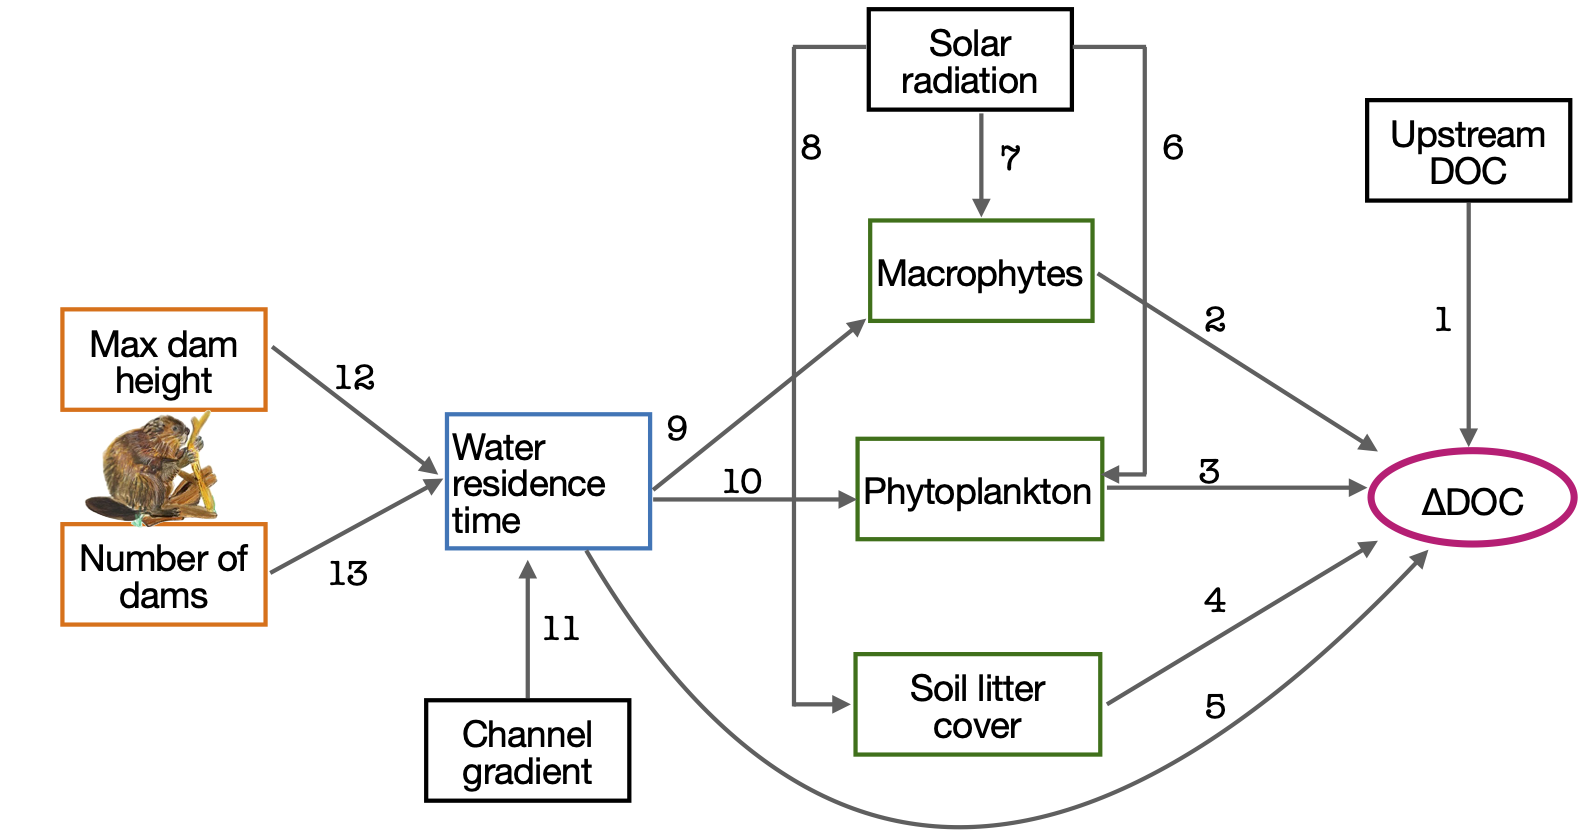
\includegraphics[width=\textwidth]{figures/media/figS1_dag_hypotheses.png}
\caption{Directed acyclic graph (DAG) of the structural causal model (SCM), with the hypothesised causal mechanisms numbered 1--13. Orange boxes: beaver-engineering variables; the blue box: stream hydrology; green boxes: primary producer variables; black boxes: parent drivers not influenced by other variables; the magenta ellipse: the outcome \(\Delta\)DOC. Each numbered edge corresponds to one tested hypothesis in Table~S1. Two further paths, 14 and 15 (upstream DOC $\rightarrow$ macrophytes, upstream DOC $\rightarrow$ phytoplankton, not drawn here), were added and tested as part of the structural sensitivity analysis and are included in the extended model (Figure 4, main document; Structural sensitivity: alternative causal structures). Beaver illustration credits to \textcopyright{} Sarah Edmonds Illustration.}\label{fig:S1}
\end{figure}

\FloatBarrier
\section*{SCM: tested hypothesis}



\setlength{\LTleft}{0pt}\setlength{\LTright}{0pt}\begingroup\small\sloppy\hyphenpenalty=0\emergencystretch=2em
\renewcommand{\arraystretch}{1.25}
\begin{longtable}{|>{\centering\arraybackslash}p{0.07\textwidth}|>{\raggedright\arraybackslash}p{0.17\textwidth}|>{\raggedright\arraybackslash}p{0.14\textwidth}|>{\raggedright\arraybackslash}p{0.48\textwidth}|}
\caption{Tested hypotheses for the structural causal model (SCM). The causal-path numbers correspond to the numbered edges of the DAG in Figure~\ref{fig:S1} (and Figure 4 of the main document).}\label{tab:S1}\\
\hline
\textbf{Causal path} & \textbf{Predictor} & \textbf{Response} & \textbf{Hypothesis} \\ \hline
\endfirsthead
\multicolumn{4}{l}{\small\textit{Table S1 (continued)}}\\
\hline
\textbf{Causal path} & \textbf{Predictor} & \textbf{Response} & \textbf{Hypothesis} \\ \hline
\endhead
\multicolumn{4}{r}{\small\textit{continued on next page}}\\
\endfoot
\endlastfoot
1 & DOC upstream & \(\Delta DOC\) & If DOC upstream increases, then \(\Delta DOC\) decreases because beaver ponds can act as sink, retaining or transforming DOC through processes such as microbial degradation, sedimentation, and photodegradation, thereby reducing downstream DOC concentrations relative to upstream inputs (Larson et al. 2007; Wohl 2013; Johnston 2014). \\ \hline
2 & Macrophytes & \(\Delta DOC\) & If macrophyte abundance increases, we expect \(\Delta DOC\) to increase because the decomposition of macrophyte biomass releases labile dissolved organic carbon, enhancing downstream concentrations (Reitsema et al. 2018). \\ \hline
3 & Phytoplankton & \(\Delta DOC\) & If phytoplankton abundance increases, then \(\Delta DOC\) increases is likely to increase, because phytoplankton contribute to DOC content through exudation during growth and release upon cell lysis, thereby enhancing downstream DOC levels relative to upstream inputs (Søndergaard et al. 1985; Sell and Overbeck 1992). \\ \hline
4 & Soil litter cover & \(\Delta DOC\) & If soil litter cover increases, then \(\Delta DOC\) increases as decomposition of litter releases dissolved organic compounds into the water (Aitkenhead et al. 1999; Cincotta et al. 2019). \\ \hline
5 & Water residence time & \(\Delta DOC\) & If water residence time increases, then \(\Delta DOC\) increases, because longer water residence times allow for more extensive microbial decomposition and processing of dissolved organic carbon, enhancing downstream DOC concentrations (Jepsen et al. 2019; Abbasi et al. 2024). \\ \hline
6 & Solar radiation & Phytoplankton & If solar radiation increases then phytoplankton abundance is expected to increase because greater light availability enhances photosynthetic rates (Reynolds 2006). \\ \hline
7 & Solar radiation & Macrophytes & If solar radiation increases, then macrophyte abundance increases because higher light availability enhances photosynthetic activity and supports plant growth (Feuchtmayr et al. 2009). \\ \hline
8 & Solar radiation & Litter cover & If solar radiation increases, as in summer, then soil litter cover decreases because lower rates of tree leaf fall coincide with enhanced decomposition driven by higher temperatures and solar radiation (Gessner et al. 1999). \\ \hline
9 & Water residence time & Macrophytes & If water residence time increases, macrophyte abundance may increase because longer residence time allows for higher nutrient retention, promoting plant growth and increasing the likelihood of macrophyte establishment and persistence (Manolaki et al. 2021). \\ \hline
10 & Water residence time & Phytoplankton & If water residence time increases, phytoplankton abundance may increase because longer residence time allows for greater nutrient retention and stabilization, which can support enhanced phytoplankton growth, particularly in systems with nutrient limitation (Finger et al. 2007). \\ \hline
11 & Channel gradient (terrain slope) & Water residence time & If valley slope increases, then water residence time decrease because steeper terrain causes water to move more quickly through the landscape, reducing the time available for subsurface and surface interactions (McGuire et al. 2005). \\ \hline
12 & Max dam height & Water residence time & If dam height increases, water residence time increases because taller dams impound more water, expanding ponded areas and slowing streamflow, which prolongs the time water remains within the stream system (Majerova et al. 2015; Dittbrenner et al. 2022). \\ \hline
13 & Number of dams & Water residence time & If the number of beaver dams increases, water residence time is expected to increase because dams slow down streamflow and create ponded areas that retain water for longer periods (Westbrook et al. 2006; Nyssen et al. 2011; Majerova et al. 2015). \\ \hline
14 & DOC upstream & Macrophytes & If DOC upstream increases, macrophyte abundance may change because a higher external carbon and nutrient supply alters light penetration and the nutrient status of the pond, in turn affecting macrophyte growth; tested as a sensitivity analysis alongside the direct path (1), not assumed a priori (Structural sensitivity: alternative causal structures). \\ \hline
15 & DOC upstream & Phytoplankton & If DOC upstream increases, phytoplankton abundance may change through the same light- and nutrient-mediated route hypothesised for macrophytes (path 14); tested as a sensitivity analysis alongside the direct path (1), not assumed a priori (Structural sensitivity: alternative causal structures). \\ \hline
\end{longtable}
\renewcommand{\arraystretch}{1}\endgroup


\FloatBarrier
\section*{Structural Causal Model: the priors}

To ensure the model was not over-constrained by prior knowledge, we used weakly informative priors for all parameters. This approach allows the data to inform the model without assuming strong beliefs about the parameter values beforehand (Figure~\ref{fig:S2}). We note, however, that for macrophytes, phytoplankton, and litter cover---variables measured in 16 of the 179 streams---we used more informative priors that incorporate established ecological knowledge about their influence on DOC concentrations (Figure~\ref{fig:S2}b), and that the two links from upstream DOC to macrophytes and phytoplankton (paths 14--15) carry a weakly informative Normal(0, 0.1) prior, expressing no directional expectation (Figure~\ref{fig:S2}c).

\begin{figure}[!htb]
\centering
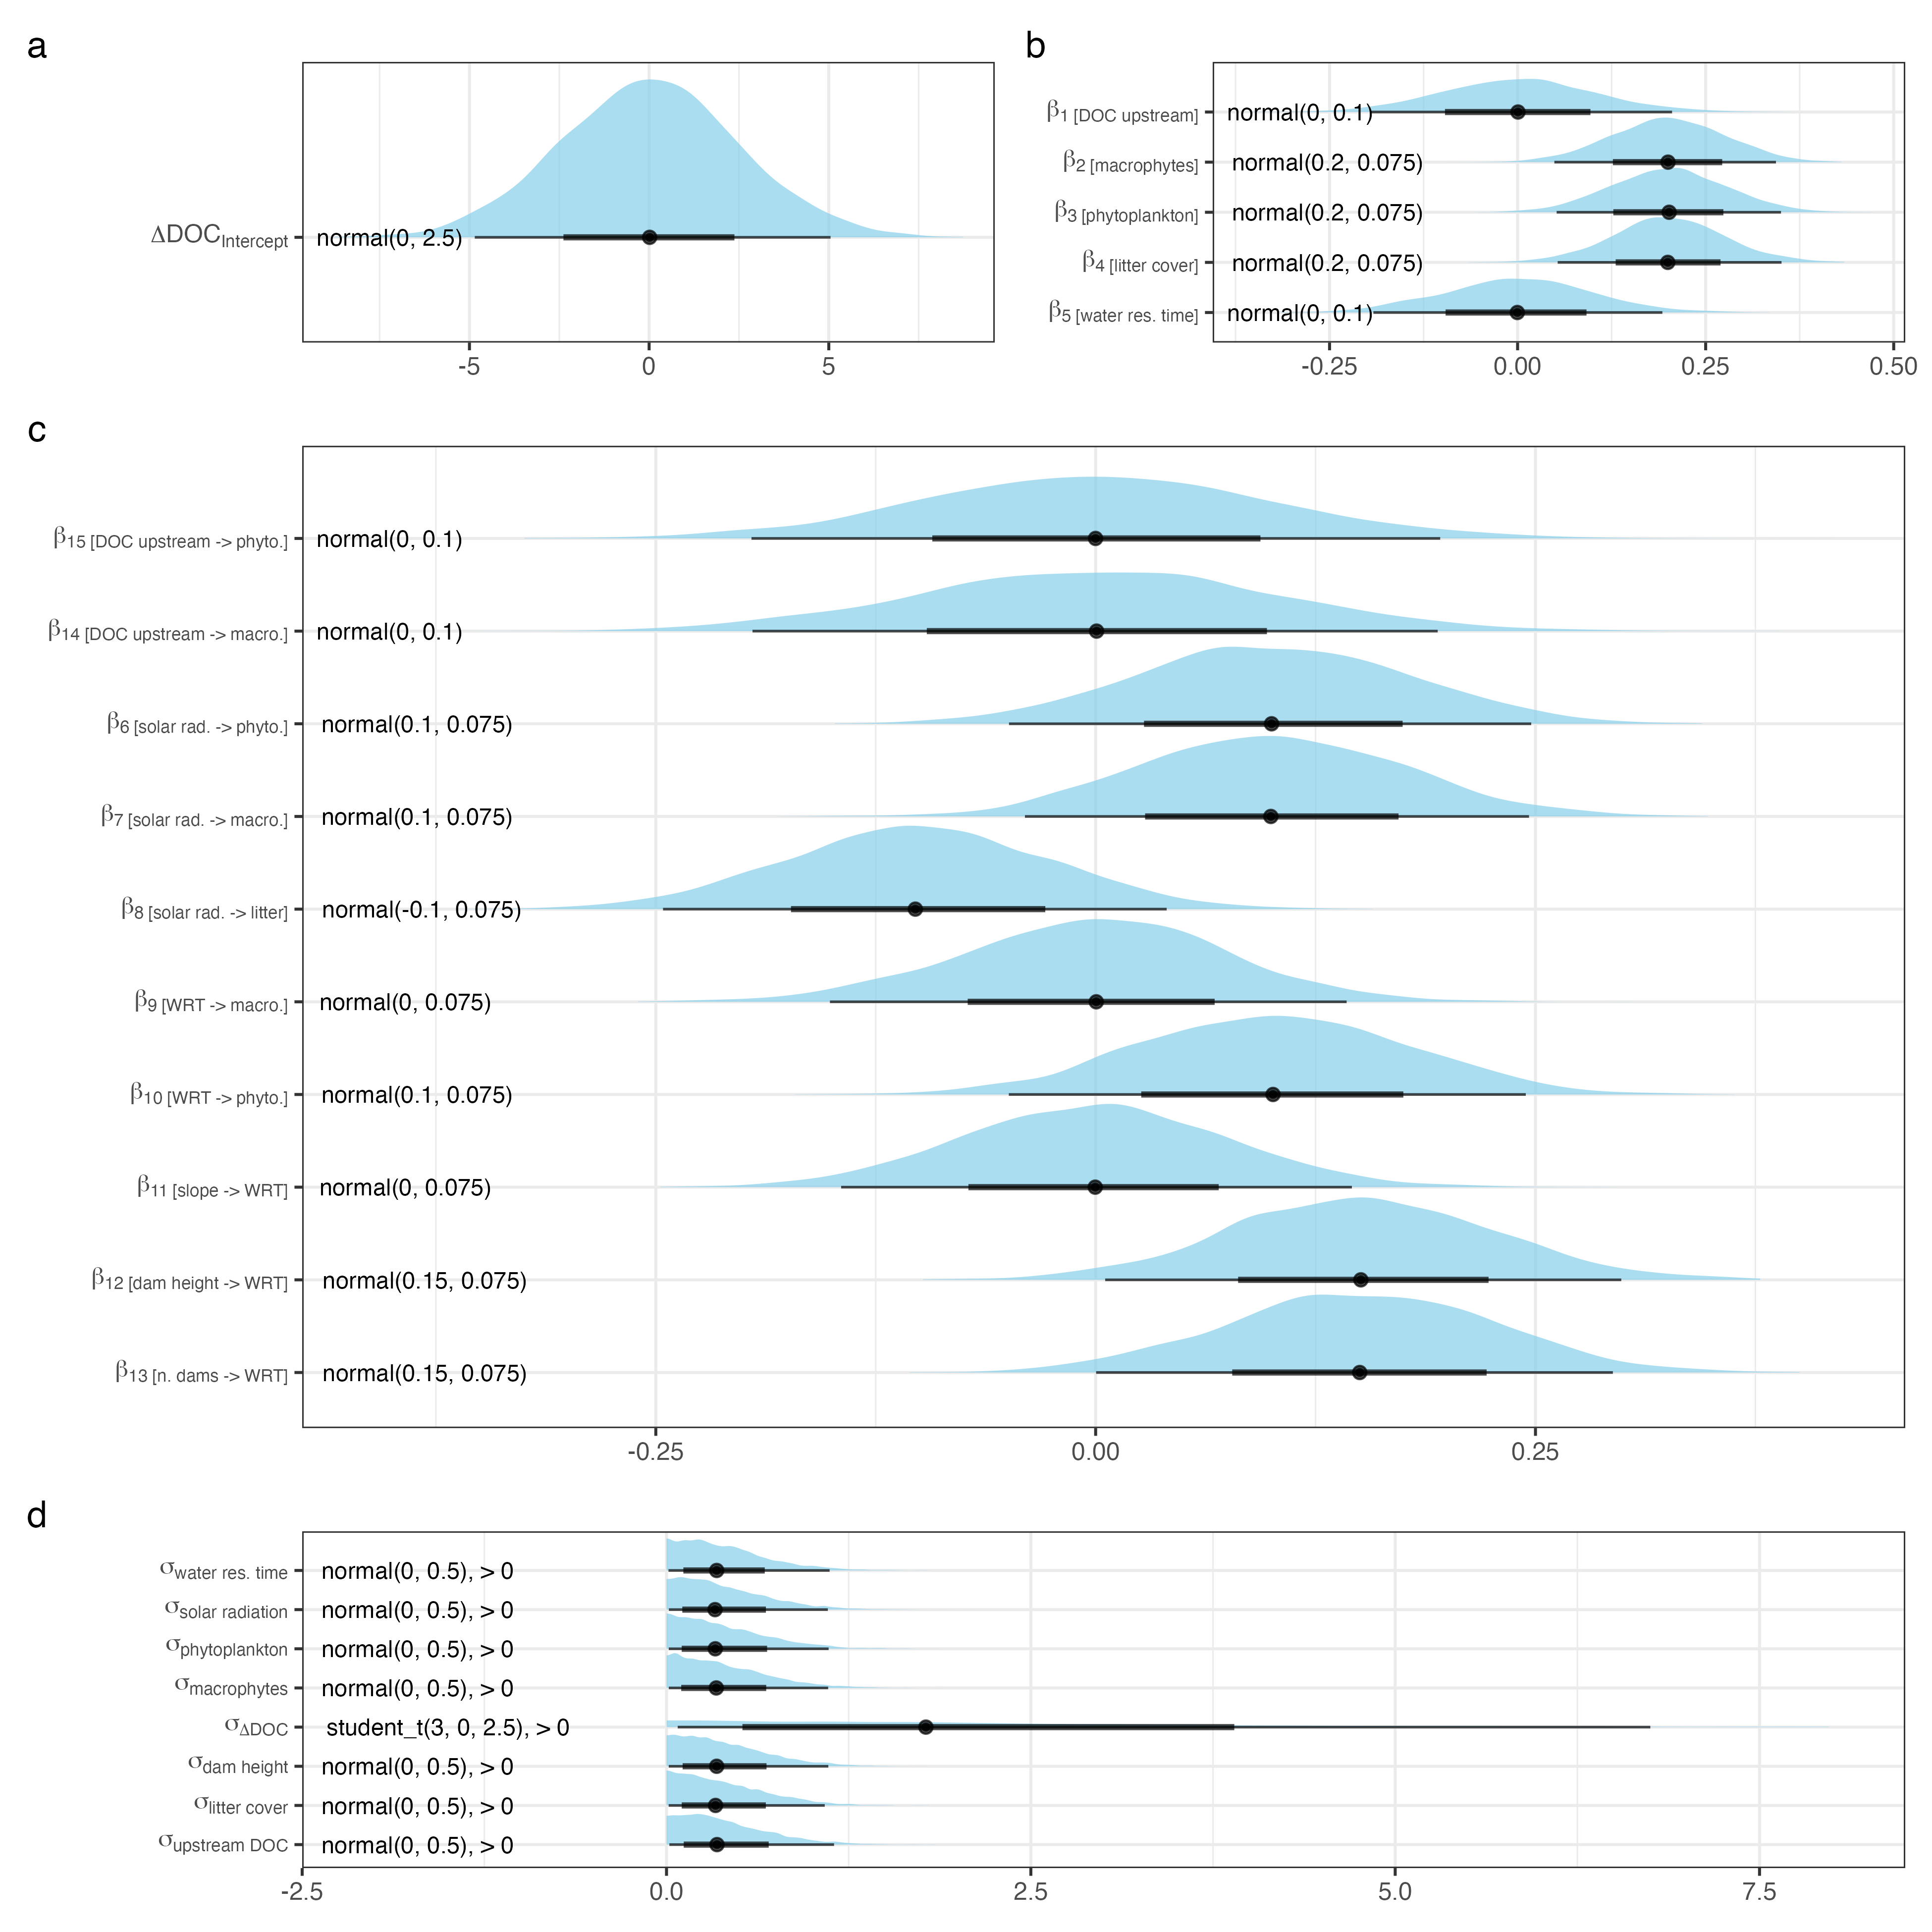
\includegraphics[width=\textwidth]{figures/media/figS2_priors.png}
\caption{Half-eye plots display the prior distributions used in the extended structural causal model (delta\_SCM\_me). The shaded areas (slabs) represent the probability density of each prior distribution, illustrating their shape and spread. The central dot indicates the median of the distribution, while the thick and thin horizontal lines represent the 66\% and 95\% credible intervals, respectively. Text labels to the left of each distribution indicate the corresponding prior specification. a) the $\Delta$DOC intercept, b) the direct effects on $\Delta$DOC (paths 1--5), c) the indirect-effect paths (6--15, including the two upstream-to-producer links 14--15), d) the residual standard deviations.}\label{fig:S2}
\end{figure}

\FloatBarrier
\section*{Structural Causal Model: the residuals}

We can evaluate the model fit by looking at the difference between observed data and their predictions. That are the residuals (\(r_{i}\)).

\begin{equation}
r_{i} = y_{i} - y_{i}^{pred}
\end{equation}

If the model is a reasonable representation of the observational process that originates the data then the residuals should look roughly randomly scattered in comparison to a horizontal line.

\begin{figure}[!htb]
\centering
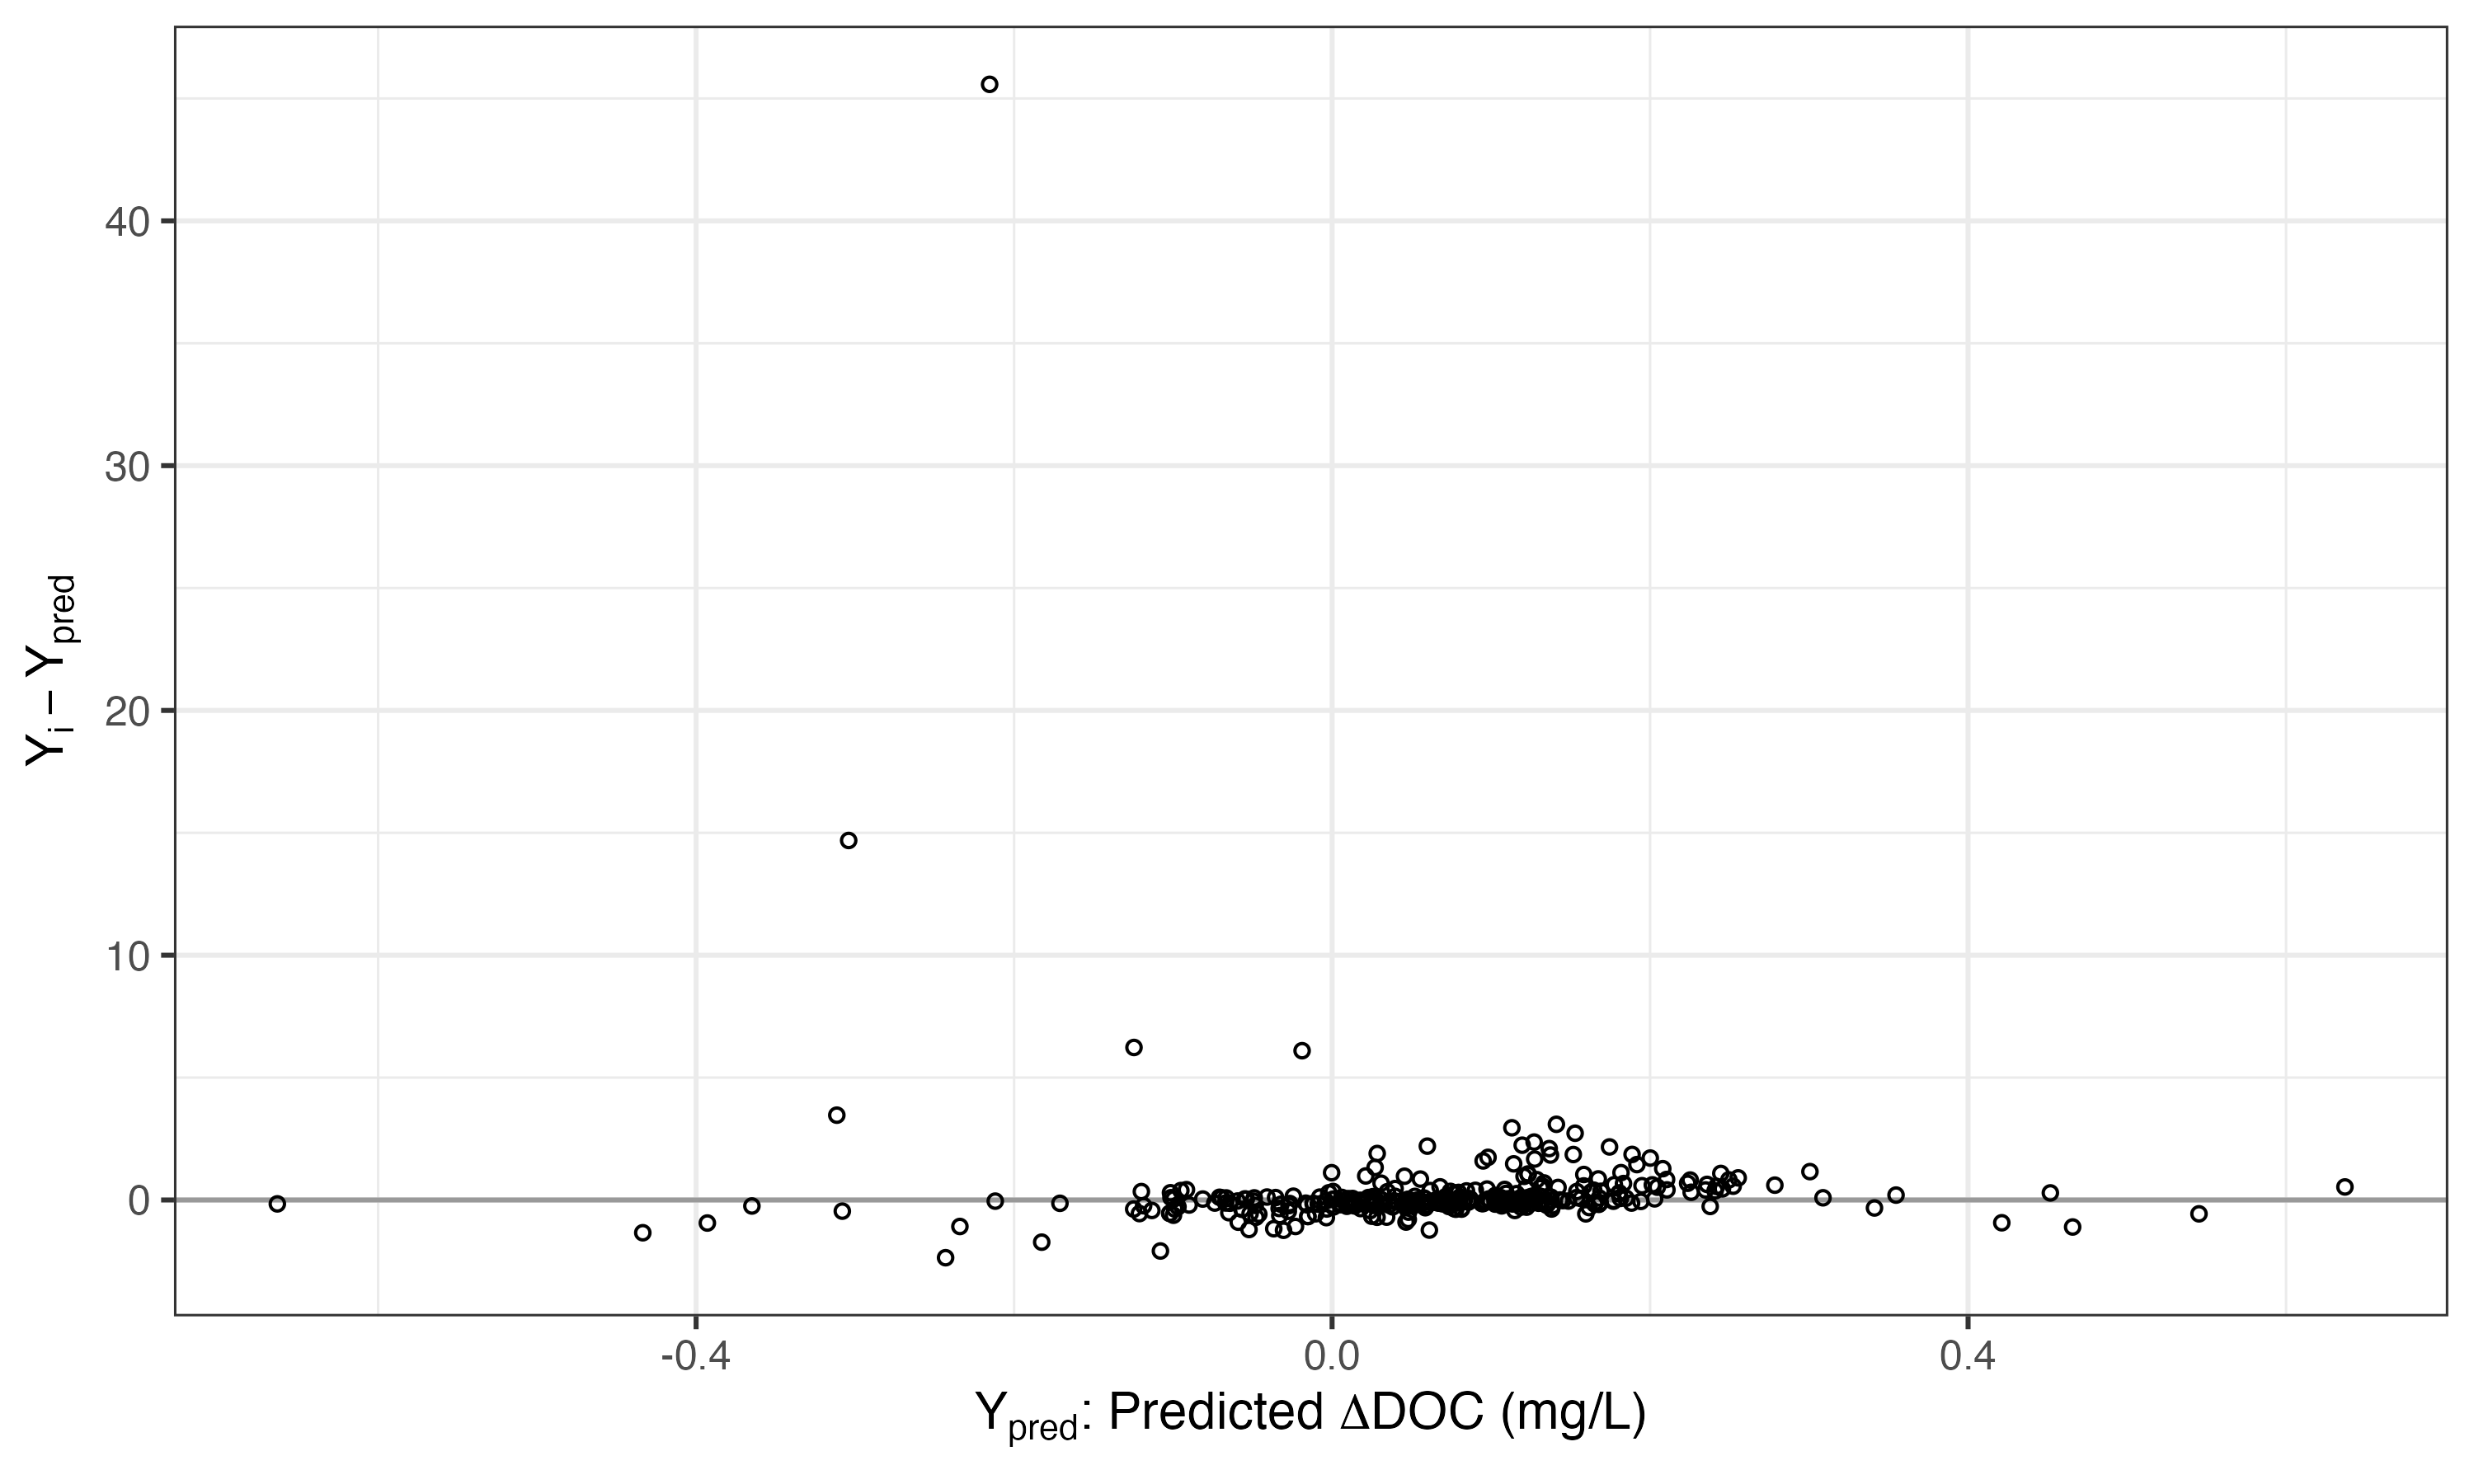
\includegraphics[width=\textwidth]{figures/media/figS3_residuals.png}
\caption{Residual plot of the extended structural causal model (delta\_SCM\_me): model-predicted $\Delta$DOC values (mg\,L$^{-1}$) against the corresponding residuals. Points represent the difference between observed and predicted values; a random scatter around zero (grey line) indicates good model fit and no systematic bias in predictions. The single point near $Y_i - Y_{pred} \approx 45$ mg L$^{-1}$ is stream RBK08's summer sampling, the largest local change in the dataset (main document, Discussion).}\label{fig:S3}
\end{figure}

\FloatBarrier
\section*{Structural Causal Model: posterior predictive checks}

Posterior predictive checks assess how well the fitted SCM model reproduces observed data by comparing the observed values to data simulated from the model's posterior predictive distribution.

\begin{figure}[!htb]
\centering
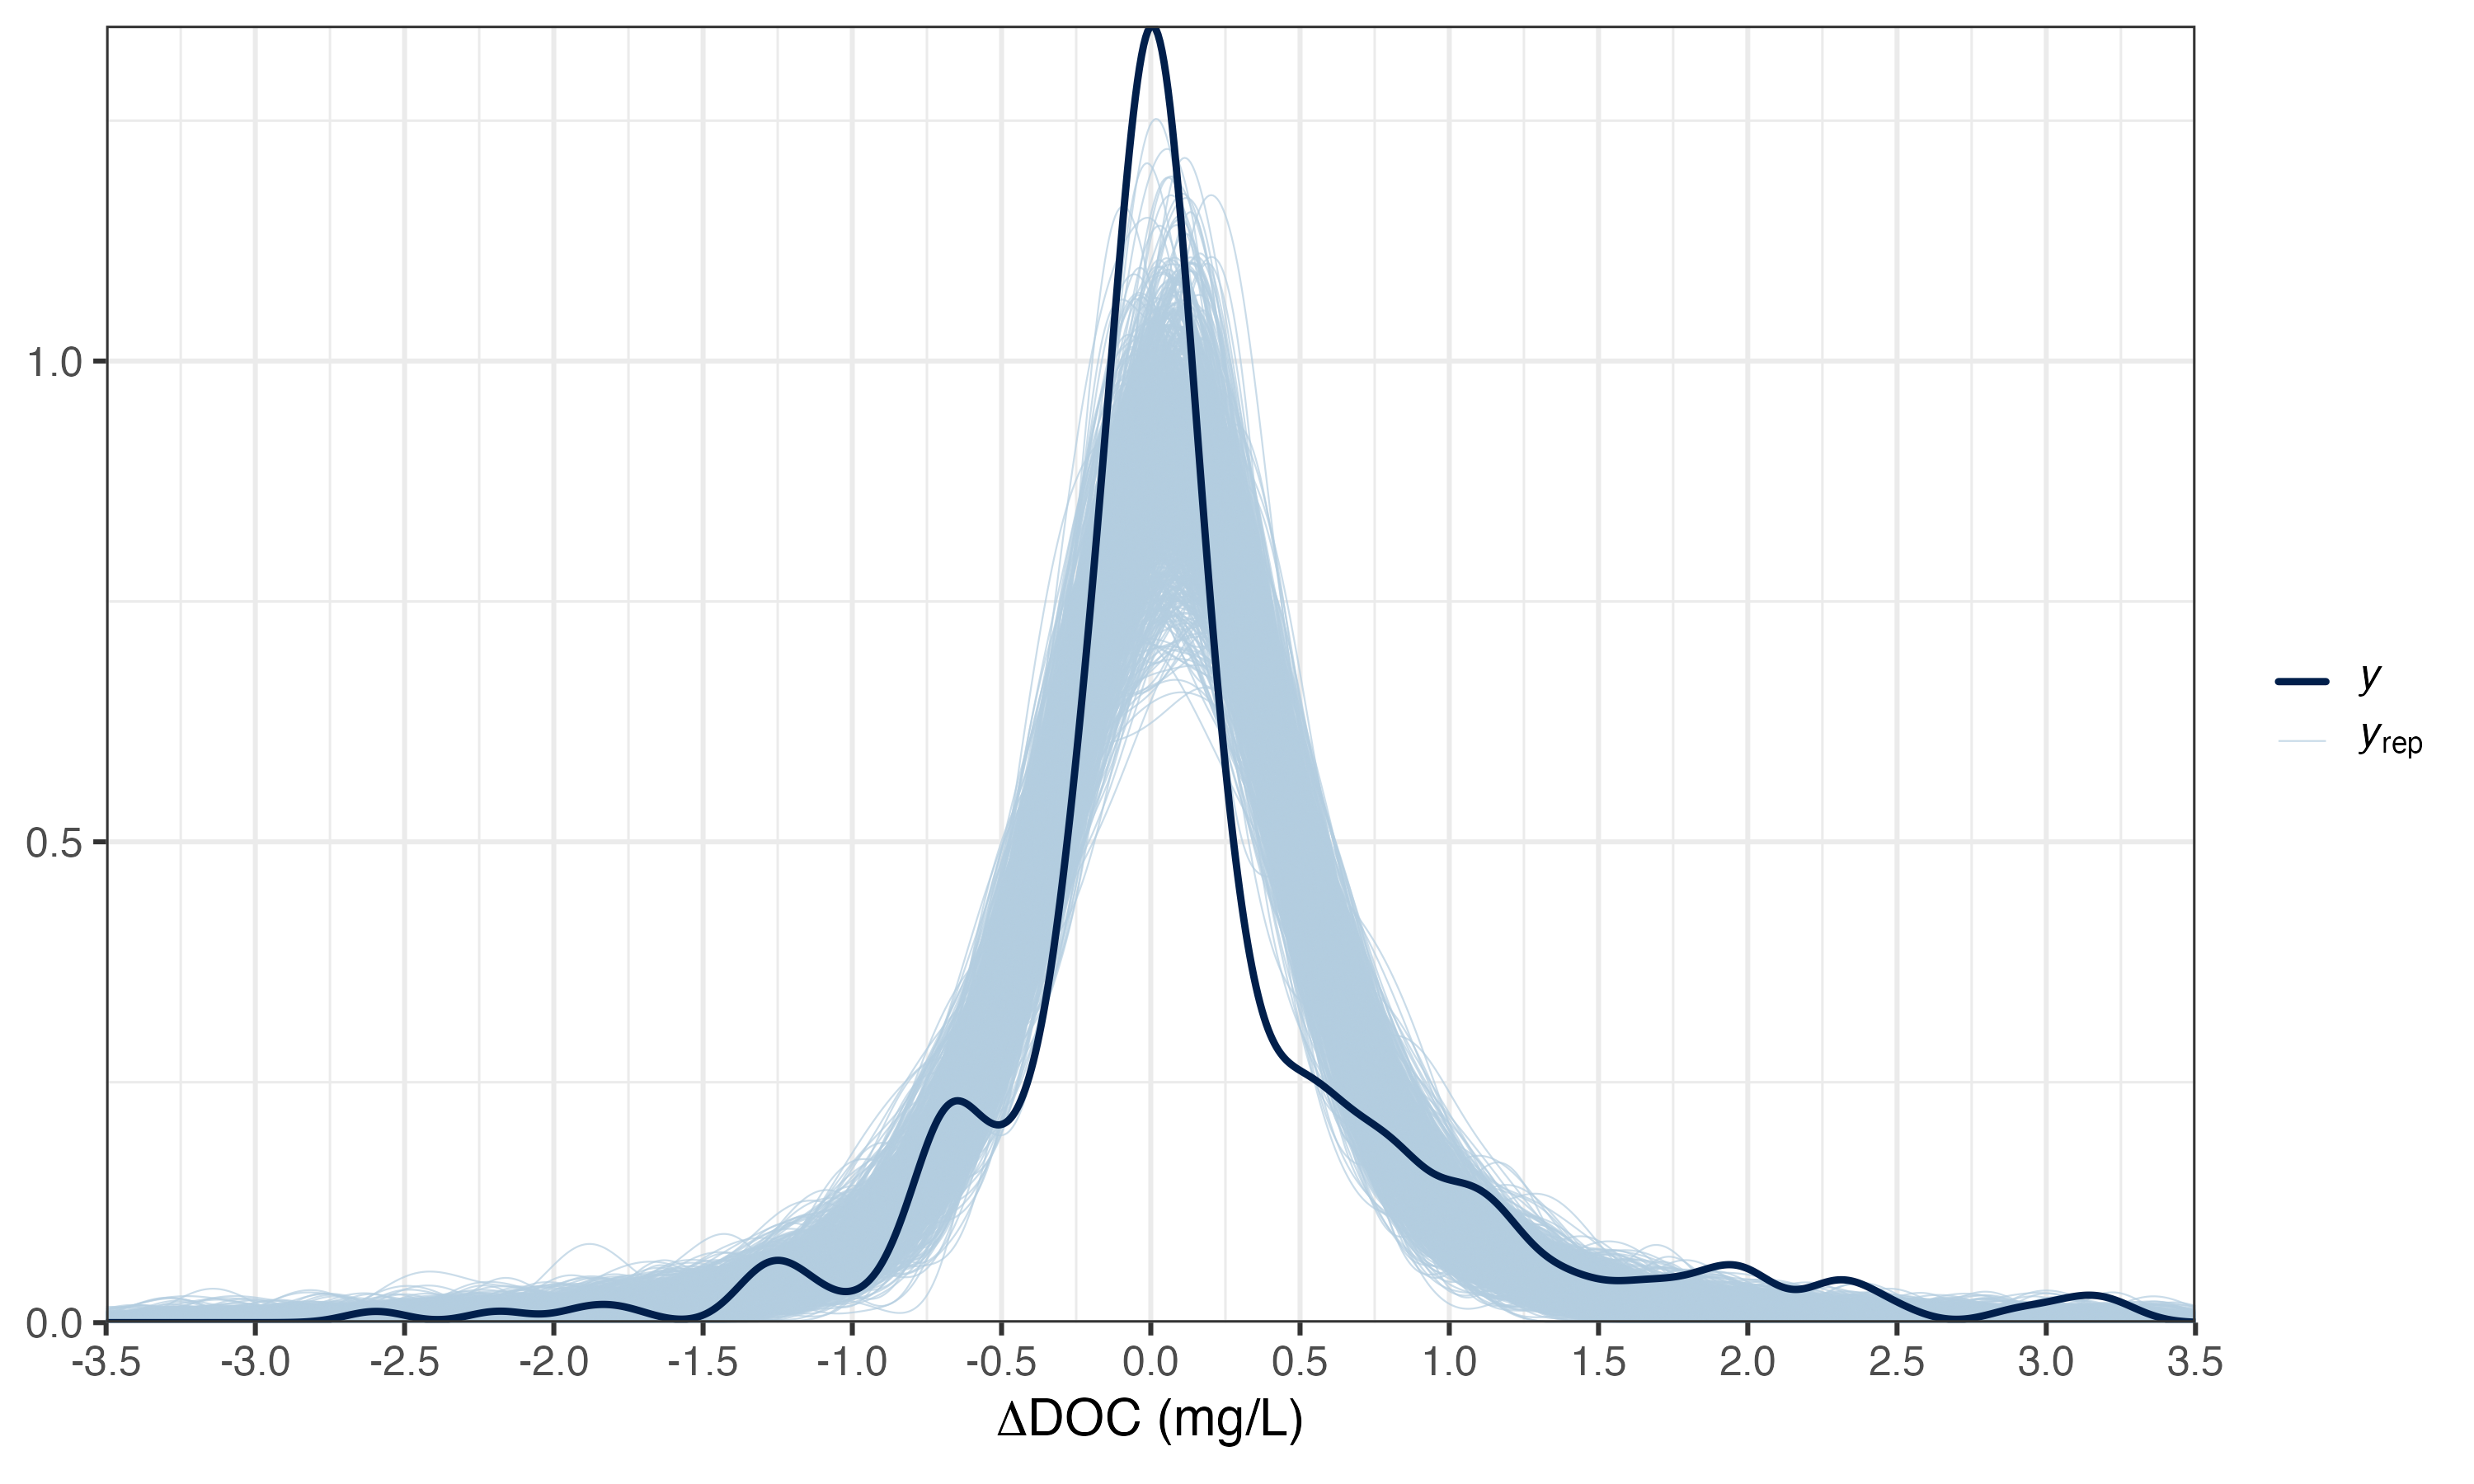
\includegraphics[width=\textwidth]{figures/media/figS4_ppc.png}
\caption{Posterior predictive check of the extended structural causal model (delta\_SCM\_me). The dark line is the observed density of $\Delta$DOC and the light lines are 1000 datasets simulated from the posterior.}\label{fig:S4}
\end{figure}

\FloatBarrier
\section*{Structural Causal Model: posterior parameters distribution}

\begin{figure}[!htb]
\centering
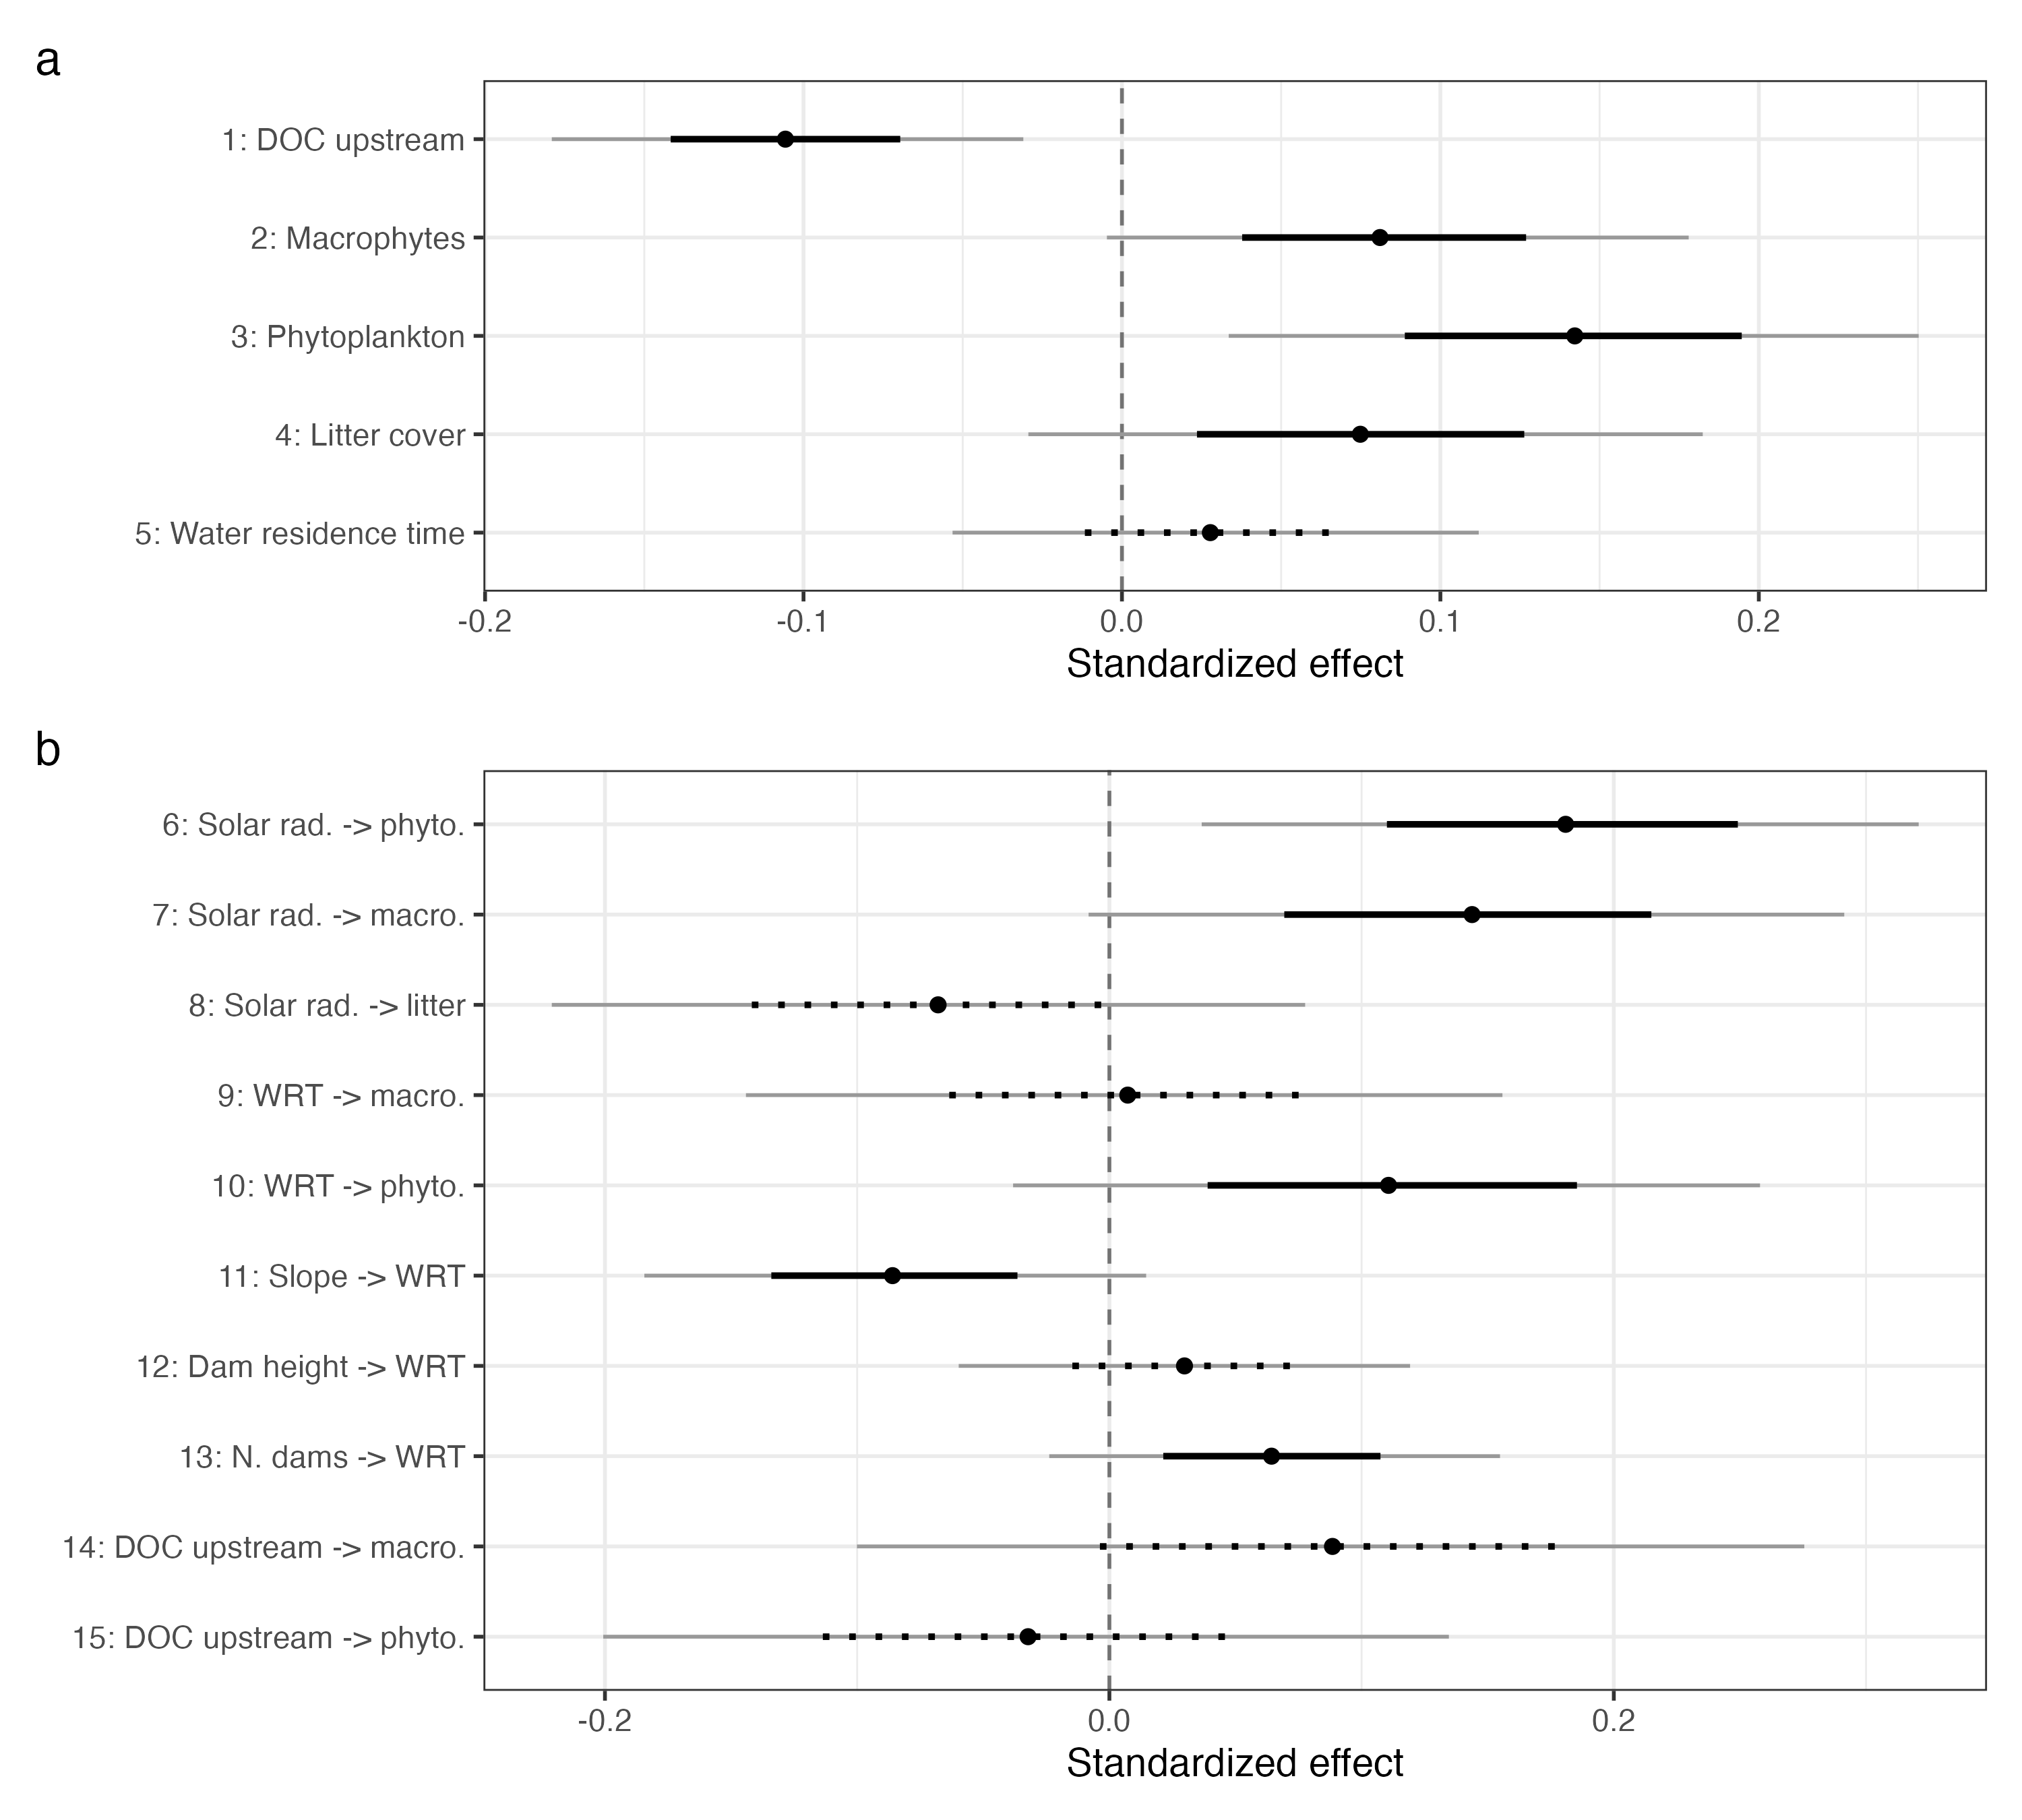
\includegraphics[width=\textwidth]{figures/media/figS5_posteriors.png}
\caption{Posterior parameter distributions of the extended structural causal model (delta\_SCM\_me). Median shown with point; 66\% and 95\% credible intervals shown with bars (solid: more than 90\% posterior probability mass on one side of zero; dotted: no-evidence). a) The direct effects on $\Delta$DOC (paths 1--5). b) The indirect-effect paths (6--15), including the two upstream-to-producer links (14, 15).}\label{fig:S5}
\end{figure}




\FloatBarrier
\section*{Structural Causal Model: stream-level classification of $\Delta$DOC}

The large variability of individual responses shown in Figure 2 (main document) can arise in two fundamentally different ways: either streams differ consistently from each other -- some being stable DOC sources, others stable sinks -- or each stream fluctuates between source, negligible and sink behaviour from one sampling occasion to the next. Distinguishing these two possibilities matters for interpretation and management: only in the first case could one map and manage ``source streams'' and ``sink streams''; the sink/negligible/source percentages of Figure 2 are probabilities per sampling and must not be read as percentages of streams. To answer this question we classified each stream individually using the extended structural causal model (delta\_SCM\_me), whose stream-level random intercept captures any consistent between-stream differences. (As a consistency check, the posterior predictive distribution of $\Delta$DOC from the SCM for a typical stream -- predictors at their mean, stream effects integrated out -- gives 12\% sink, 76\% negligible and 13\% source responses, in close agreement with the season-specific measurement-error model of Figure 2.) For each upstream--downstream unit (this model's site variable resolves 179 units from a few streams sampled as more than one separately sampled beaver-dam sequence; the main text's 158 analysed streams count the concentration-based models of Q1 and Q3, which pool multiple sequences at the same stream) we computed the posterior distribution of the expected $\Delta$DOC (population-level effects plus the stream-level intercept, averaged over the unit's observations; 2,000 posterior draws) and assigned each unit to the region (sink $< -0.5$ mg L$^{-1}$, ROPE $\pm 0.5$ mg L$^{-1}$, source $> 0.5$ mg L$^{-1}$) that held the majority of its posterior mass. The expected $\Delta$DOC of every unit fell within the ROPE (posterior medians from $-0.41$ to $0.46$ mg L$^{-1}$; median width of the 90\% credible interval 0.41 mg L$^{-1}$; Figure~\ref{fig:S6}), reflecting the small average effect (intercept 0.00 mg L$^{-1}$; 95\% BCI $-0.11$; 0.12) and the small between-stream standard deviation (0.05 mg L$^{-1}$; 95\% BCI 0.00; 0.14). The answer is therefore the second possibility: no stream shows consistent source or sink behaviour, and the heavy-tailed posterior predictive distribution of Figure 2 captures the variability of individual samplings around a null average rather than stable stream-level differences.

\begin{figure}[!htb]
\centering
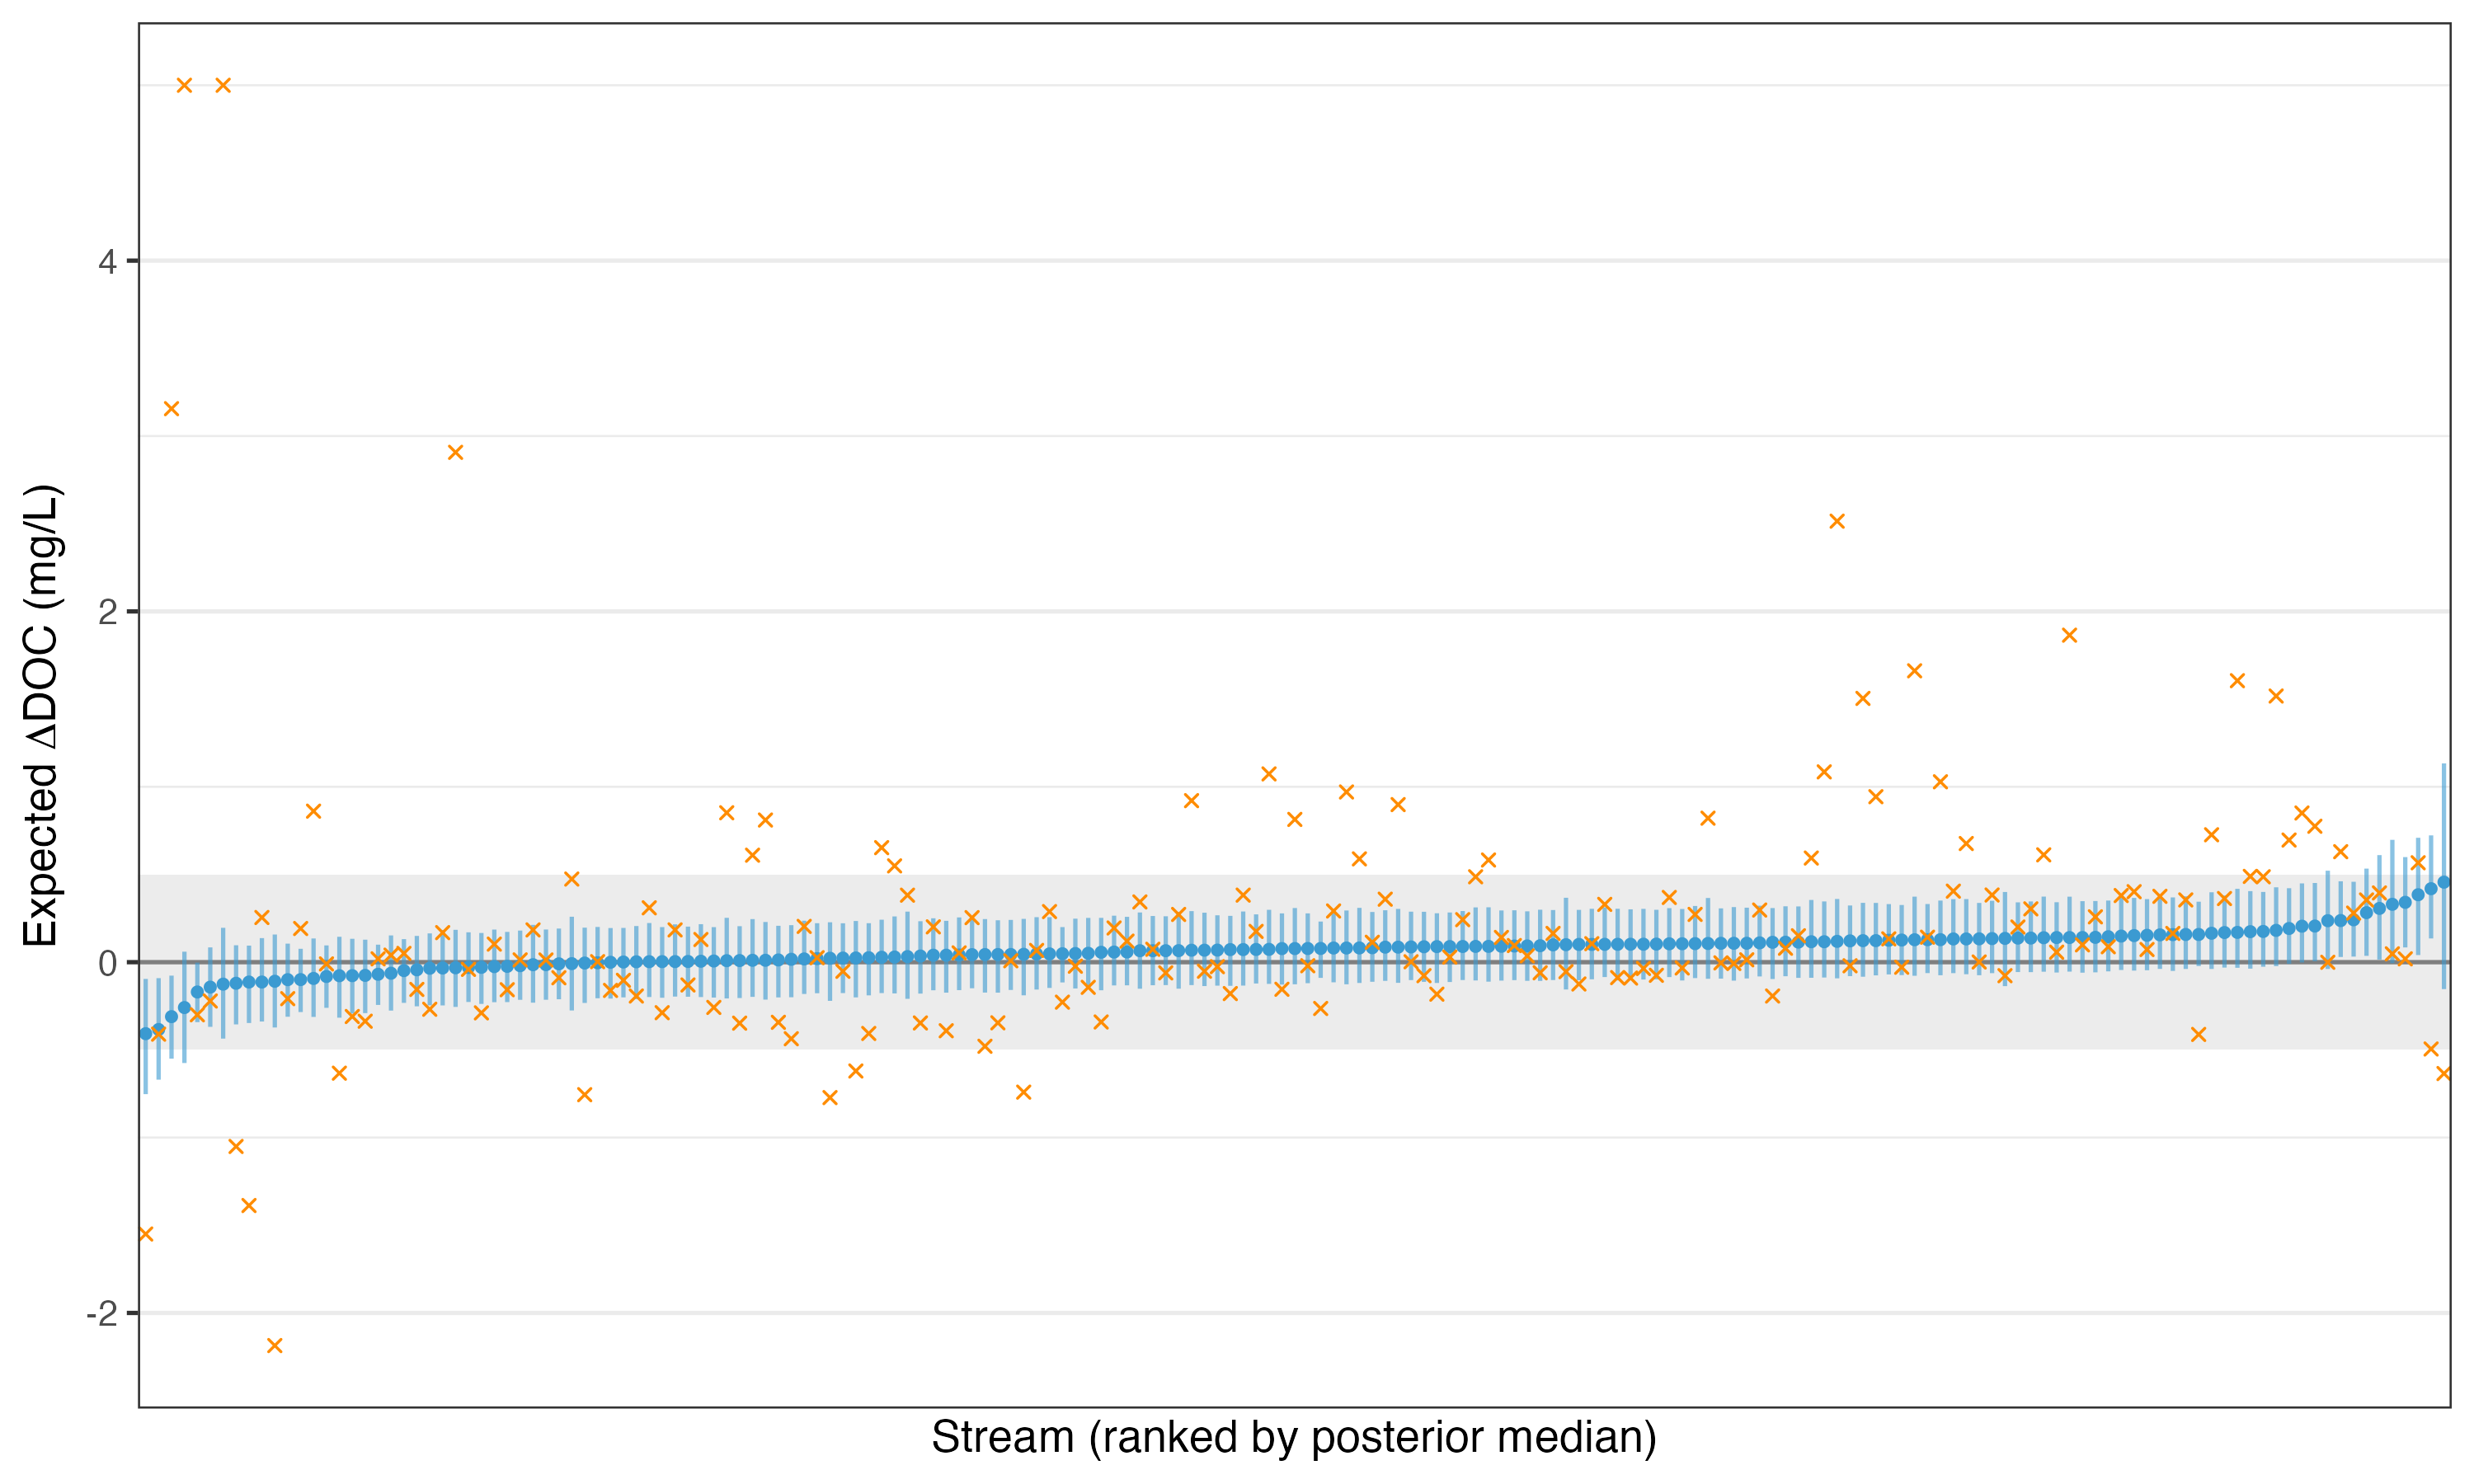
\includegraphics[width=\textwidth]{figures/media/figS7_site_level.png}
\caption{Stream-level $\Delta$DOC under the extended structural causal model (delta\_SCM\_me). Blue points and bars: posterior median and 90\% credible interval of the model-based expected $\Delta$DOC of each unit (ranked by posterior median). Orange crosses: observed stream-averaged $\Delta$DOC, shown for reference (two values above 5 mg L$^{-1}$, both stream RBK08, are clipped at 5 mg L$^{-1}$). The grey band is the region of practical equivalence ($\pm 0.5$ mg L$^{-1}$).}\label{fig:S6}
\end{figure}


\FloatBarrier
\section*{Structural Causal Model: total effects of the exogenous drivers on $\Delta$DOC}

The edges of the SCM (Figure 4, main document) are direct, path-specific effects. To summarize the overall influence of each exogenous driver on $\Delta$DOC we computed its \emph{total effect} as the sum of the products of the coefficients along every open causal path from the driver to $\Delta$DOC (e.g., for the number of dams: dams $\rightarrow$ WRT $\rightarrow$ $\Delta$DOC, dams $\rightarrow$ WRT $\rightarrow$ macrophytes $\rightarrow$ $\Delta$DOC, and dams $\rightarrow$ WRT $\rightarrow$ phytoplankton $\rightarrow$ $\Delta$DOC), evaluated on each posterior draw (path tracing; Hayes 2018). Under the extended model, upstream DOC's total effect additionally includes the two new paths through macrophytes and phytoplankton (14, 15). All effects are on the standardized scale (change in $\Delta$DOC, in standard deviations, per standard deviation of the driver).

Upstream DOC concentration had the largest total effect ($-0.10$; 90\% BCI: $-0.16$; $-0.05$; $P(\beta<0) = 1.00$), followed by solar radiation, which acts through all three primary-producer mediators ($+0.04$; 90\% BCI: 0.01; 0.07; $P(\beta>0) = 0.99$). The total effect of water residence time ($+0.05$; 90\% BCI: $-0.02$; 0.11; $P(\beta>0) = 0.88$) was positive but less certain. The total effects of the beaver-engineering variables, which act only through water residence time, were small: number of dams $+0.00$ (90\% BCI: $-0.00$; 0.01; $P(\beta>0) = 0.82$) and maximum dam height $+0.00$ (90\% BCI: $-0.00$; 0.01; $P(\beta>0) = 0.68$); channel gradient had a small negative total effect ($-0.00$; 90\% BCI: $-0.01$; 0.00; $P(\beta<0) = 0.84$). Adding the two upstream-to-producer paths changes none of these conclusions: the new indirect route from upstream DOC through the producers is an order of magnitude smaller than its direct effect (main document, Results), so the total effect above is carried almost entirely by that direct path. Hence, the direction of the beaver-mediated DOC change is set primarily by the external context of the pond (incoming DOC load and light availability for primary producers), whereas the structural characteristics of the dam complex modulate it only weakly via water residence time (Figure~\ref{fig:S7}).

\begin{figure}[!htb]
\centering
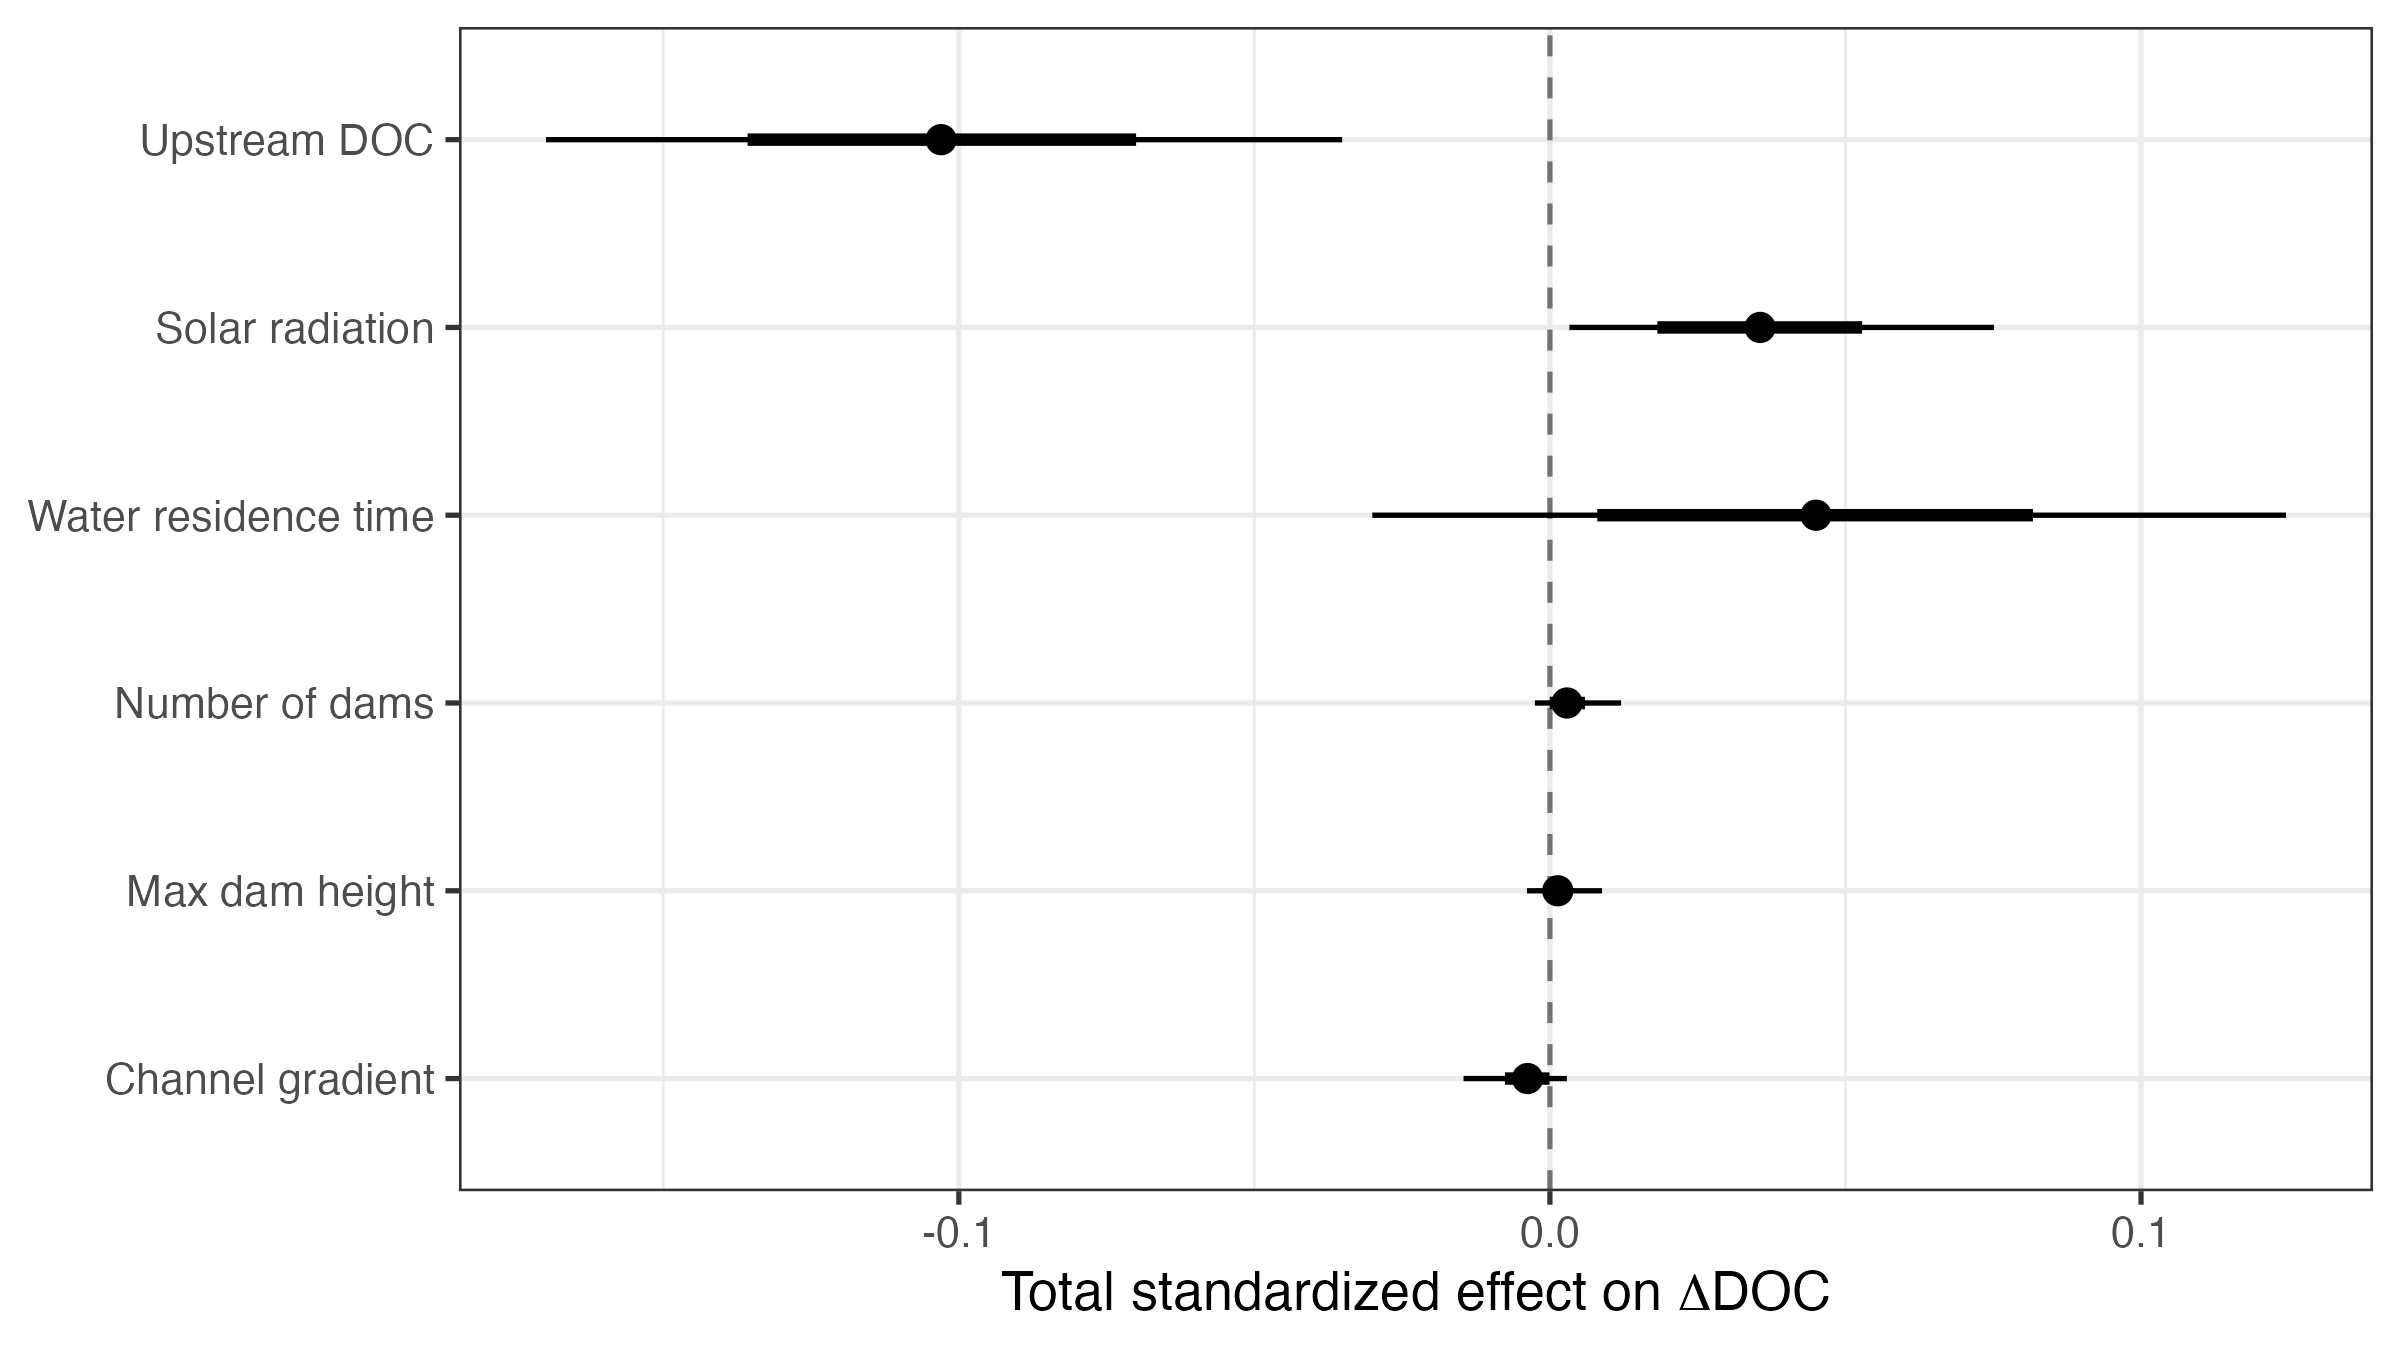
\includegraphics[width=0.9\textwidth]{figures/media/figS8_total_effects.png}
\caption{Posterior distributions of the total (standardized) effect of each exogenous driver on $\Delta$DOC under the extended structural causal model (delta\_SCM\_me), obtained by tracing all open causal paths, including the two new upstream-to-producer paths. Points: posterior means; thick and thin bars: 66\% and 95\% credible intervals.}\label{fig:S7}
\end{figure}

\FloatBarrier
\section*{Alternative structural causal model: lateral stream--wetland connectivity}

Because a DAG encodes a specific set of causal assumptions, we also tested an alternative, extended SCM that adds one causal path to the main SCM (Figure~\ref{fig:S1}): path 14, from the lateral connectivity between the stream and adjacent wetlands to water residence time (WRT; Figure~\ref{fig:S8}). Our hypothesised mechanism is that a hydrologically connected wetland acts as an off-channel transient-storage zone: water moves laterally into and out of this storage compartment, extending the time it resides in the reach before continuing downstream (transient-storage theory; Bencala and Walters 1983; Wegener et al. 2017; Wohl 2021). We therefore hypothesised that beaver-pond WRT increases with the degree of lateral stream--wetland connectivity and, consequently, that connectivity indirectly influences $\Delta$DOC via WRT and the primary producers.

\begin{figure}[!htb]
\centering
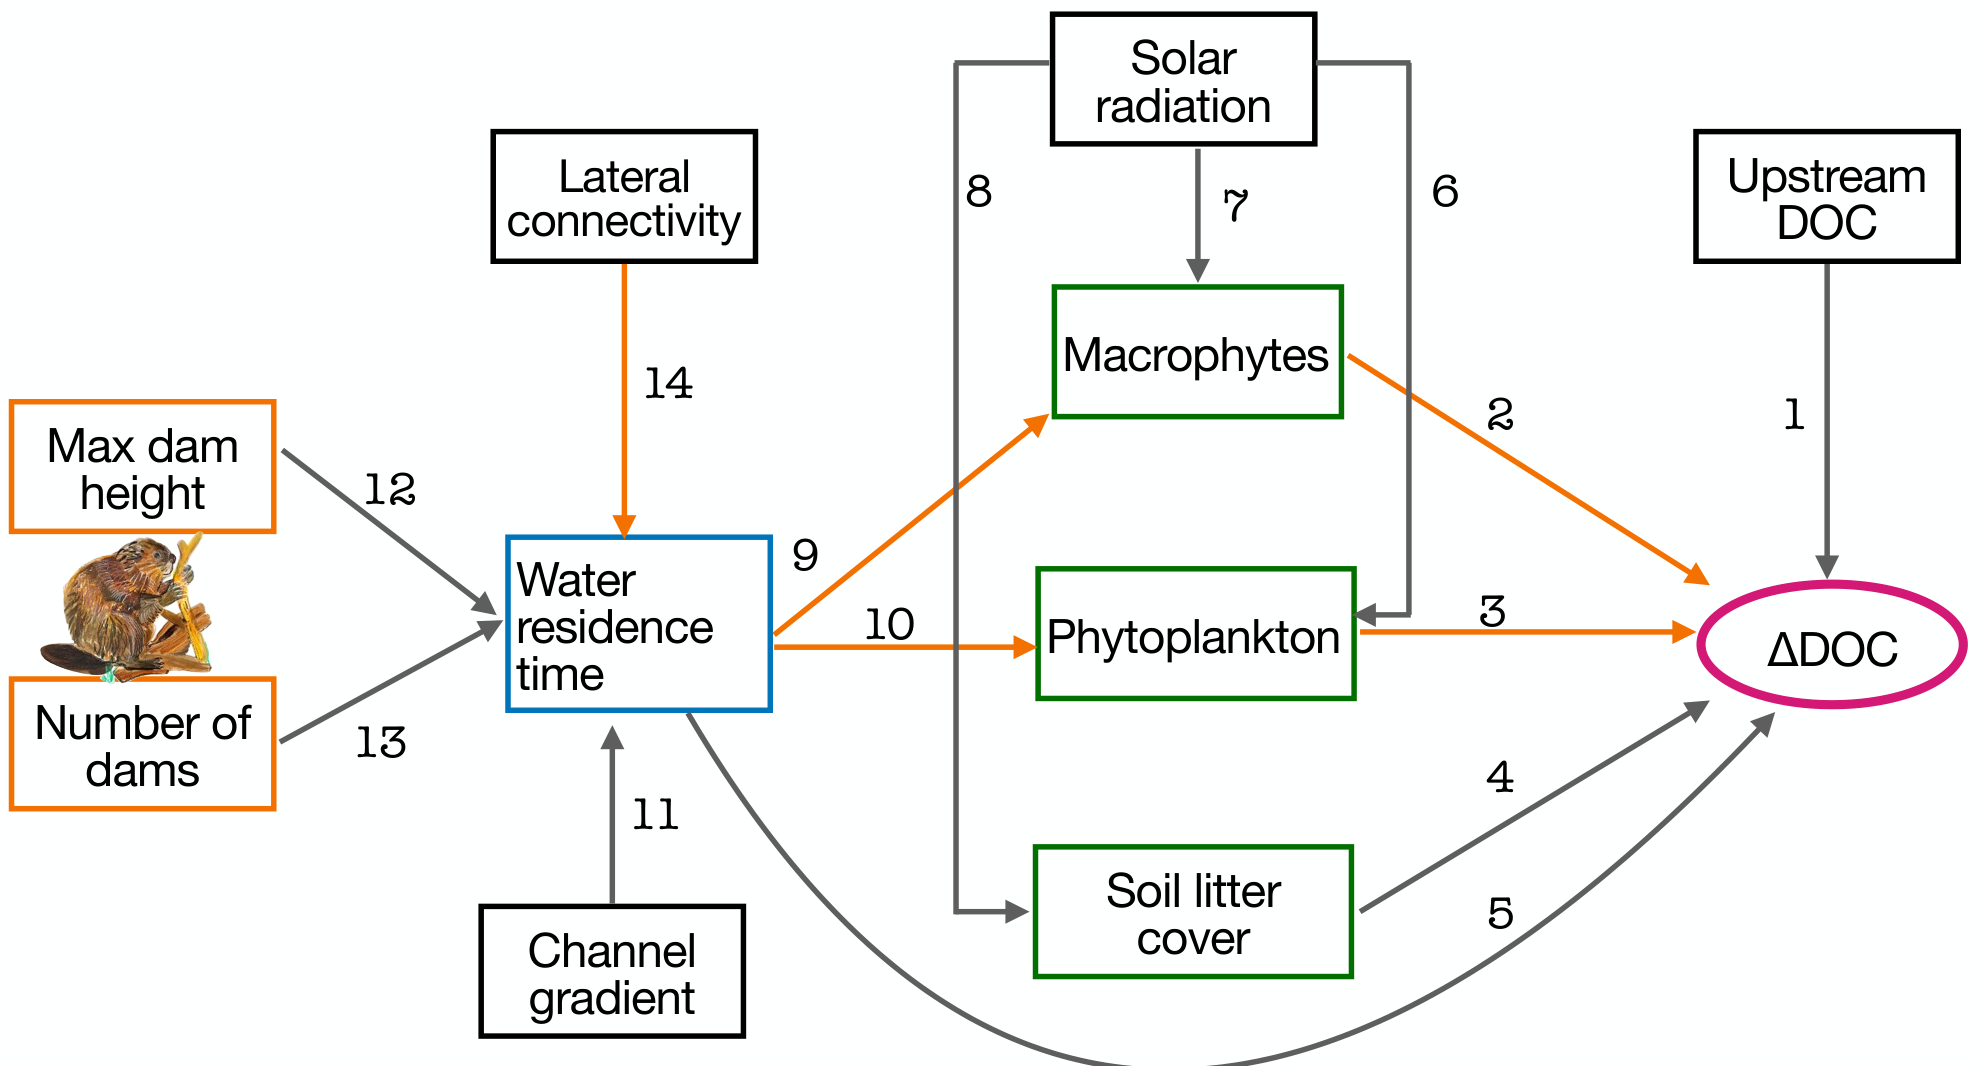
\includegraphics[width=\textwidth]{figures/media/figS8_dag_connectivity_alt.png}
\caption{Extended directed acyclic graph (DAG) of the alternative SCM. It is identical to the main SCM (Figure~\ref{fig:S1}) except for the additional causal path 14, connecting lateral stream--wetland connectivity to water residence time. Orange edges mark the open front-door paths through which the total causal effect of lateral connectivity flows to $\Delta$DOC (paths 14 $\rightarrow$ 9 $\rightarrow$ 2, 14 $\rightarrow$ 10 $\rightarrow$ 3, and 14 $\rightarrow$ 5).}\label{fig:S8}
\end{figure}

\paragraph{Connectivity variable.} For each site, we first determined whether a wetland was present within a 50~m buffer around the river reach between the upstream and downstream sampling locations, using the wetland layer (marshes, bogs, swamp forests, wet meadows, floodplains and fens) of the swissTLM3D topographic landscape model (SwissTopo 2024). For sites with a wetland, we then assessed visually on the swisstopo maps and orthophotos whether the wetland was hydrologically connected to the river water, or separated from it by roads, trails, tree lines or other barriers. Each site was thereby assigned to one of three categories: \emph{No wetland} (no wetland within the buffer; $n = 136$ sites), \emph{Wetland, not connected} (wetland present but not directly connected to the river; $n = 11$), and \emph{Wetland, connected} (wetland present and directly connected to the river; $n = 13$). Twenty-two sites could not be classified and were excluded from this analysis. Note that most of these wetlands are themselves strongly influenced by beaver damming and would likely not exist without beavers.

\paragraph{Identification: why the full SCM does not need to be re-fitted.} We encoded the extended DAG with the \emph{dagitty} R package (function \texttt{dagitty()}) and queried it with \texttt{adjustmentSets(dag, exposure = "lateral\_connectivity", outcome = "delta\_DOC", effect = "total")}, which returned the empty set, and \texttt{paths(dag, "lateral\_connectivity", "delta\_DOC")}, which lists the open paths (orange in Figure~\ref{fig:S8}). The empty adjustment set follows from the structure of the DAG: lateral connectivity has no parents (it is exogenous), so no back-door (confounding) path into $\Delta$DOC exists, and its entire causal influence flows forward through its single child, WRT. For the same reason the total effect of WRT on $\Delta$DOC is identified without adjustment. Consequently, the estimand ``total effect of connectivity on $\Delta$DOC'' equals the product of two unconfounded quantities -- the effect of connectivity on WRT and the total effect of WRT on $\Delta$DOC -- and a parsimonious model containing only the WRT equation and a $\Delta$DOC-on-WRT equation identifies it exactly. Re-fitting the entire eight-response SCM would leave this estimand unchanged (the mediator equations for macrophytes and phytoplankton are not needed when the mediated effect is captured through the total WRT $\rightarrow$ $\Delta$DOC path), while adding substantial computational cost and imputation machinery for variables that are irrelevant to the query. We therefore fitted the following two-equation Bayesian model (plus an intercept-only equation to impute missing dam heights) in \emph{brms}:

\begin{equation}
\begin{aligned}
\textbf{Outcome:} \quad \Delta \text{DOC}_i \mid \text{mi}(0.283) &\sim \text{Student-}t(\nu, \mu_i, \sigma_{\Delta \text{DOC}}), \quad \mu_i = \alpha + \beta_5 \cdot \text{WRT}_i + u_{site[i]} \\[0.5em]
\textbf{Mediator:} \quad \text{WRT}_i \mid \text{mi()} &\sim \mathcal{N}(\eta_i, \sigma_{\text{WRT}}) \\
\eta_i &= \beta_{13} \text{NDams}_i + \beta_{12} \text{DamHeight}_i + \beta_{11} \text{Slope}_i + \gamma_{c[i]} + \beta_{s} \text{Solar}_i \\[0.5em]
\textbf{Priors:} \quad \alpha &\sim \mathcal{N}(0, 2.5), \quad \beta_5 \sim \mathcal{N}(0, 0.1), \quad u_{site} \sim \mathcal{N}(0, \sigma_{site}), \quad \sigma_{site} \sim \mathcal{N}(0, 2) \\
\beta_{12}, \beta_{13} &\sim \mathcal{N}(0.15, 0.075), \quad \beta_{11}, \beta_{s} \sim \mathcal{N}(0, 0.075), \quad \gamma_{c} \sim \mathcal{N}(0, 1) \\
\sigma_{\Delta \text{DOC}} &\sim \text{Student-}t(3, 0, 2.5), \quad \sigma_{\text{WRT}} \sim \mathcal{N}(0, 0.5), \quad \nu \sim \text{Gamma}(2, 0.1)
\end{aligned}
\label{eq:altscm}
\end{equation}

where $\gamma_{c}$ are the three connectivity-level coefficients (\emph{No wetland} as reference for the contrasts) and the shared parameters carry the same informative priors as in the main SCM (Equation~4, main document); the measurement error of $\Delta$DOC (0.283 mg L$^{-1}$) and the imputation of missing WRT and dam-height values (\texttt{mi()}) are handled as in the main SCM. Four chains were run (R-hat $\le 1.005$; 310 observations). The total effect of each connectivity level on $\Delta$DOC was computed on each posterior draw as the product of the connectivity $\rightarrow$ WRT contrast and the WRT $\rightarrow$ $\Delta$DOC coefficient (path tracing, as for Figure~\ref{fig:S7}).

\paragraph{Results.} Relative to sites without wetland, the presence of an unconnected wetland increased WRT by 0.23 standardized units (90\% BCI: $-0.15$; 0.61; $P(\beta>0) = 0.84$) and a connected wetland by 0.00 (90\% BCI: $-0.36$; 0.36). The WRT $\rightarrow$ $\Delta$DOC path was positive but weak (0.07; 90\% BCI: 0.00; 0.14). The resulting total effects of connectivity on $\Delta$DOC were negligible: 0.02 (90\% BCI: $-0.01$; 0.06) for unconnected and 0.00 (90\% BCI: $-0.03$; 0.03) for connected wetlands (Figure~\ref{fig:S9}). We therefore found no evidence that lateral stream--wetland connectivity modifies the beaver-mediated DOC change through the water-residence-time pathway. Given that only 7\% and 6\% of sites fell into the connected and unconnected wetland categories, we regard this result as power-limited rather than as strong evidence of absence of an effect. Importantly, the estimates of the remaining paths were consistent with those of the main SCM (Figure~4, main manuscript), indicating that our main conclusions are robust to this alternative causal structure.

\begin{figure}[!htb]
\centering
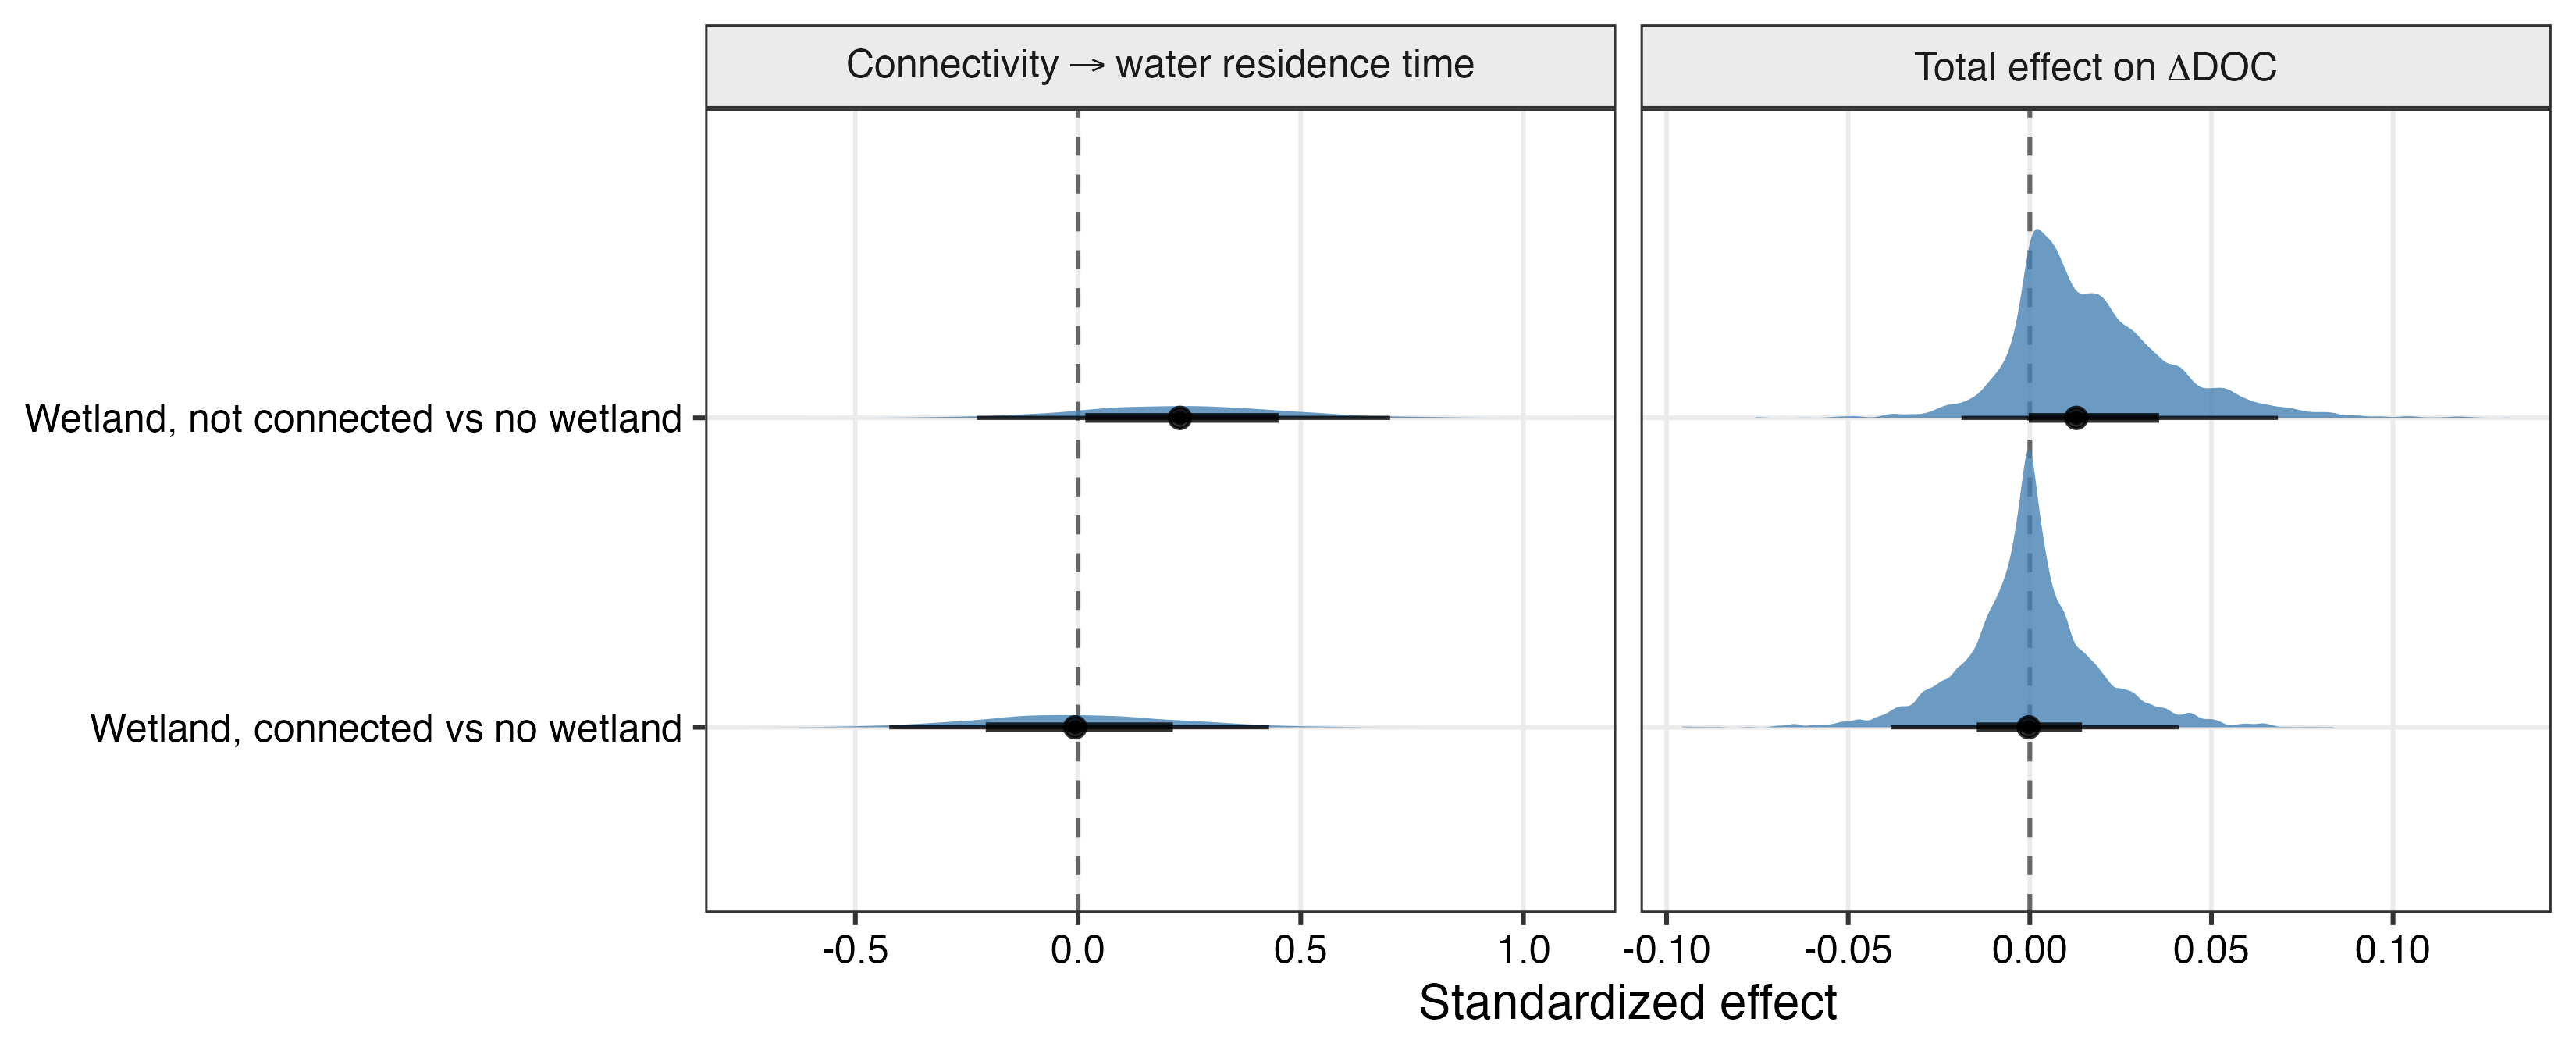
\includegraphics[width=\textwidth]{figures/media/figS9_connectivity.png}
\caption{Posterior effects of lateral stream--wetland connectivity (relative to sites without wetland) on water residence time (left) and the total mediated effect on $\Delta$DOC (right), controlling for beaver-dam variables, channel gradient and solar radiation. Points: posterior medians; thick and thin bars: 66\% and 95\% credible intervals. The dashed line marks zero.}\label{fig:S9}
\end{figure}

\FloatBarrier
\section*{Structural sensitivity: alternative causal structures}

The main SCM (Figure~4, main document) rests on causal assumptions the data cannot fully verify: the arrows drawn, the arrows left out, and the absence of unmeasured common causes. We tested four DAGs, all sharing the same mediator core: \emph{DAG 0}, the reported model, including the two causal links from upstream DOC to the primary producers and the measurement error on upstream DOC; \emph{DAG 1}, with the two upstream-to-producer links removed (the structure used before this sensitivity analysis was added); \emph{DAG 2}, adding a direct path from solar radiation to downstream DOC (photodegradation), bypassing the producers; and \emph{DAG 3}, adding season as an unblocked common cause of the producers and of downstream DOC. Each structure implies a different set of conditional independencies among the measured variables, which can be checked directly on the data (\emph{dagitty} R package); a failed independence that only one alternative structure implies is evidence for that alternative.

\begin{figure}[!htb]
\centering
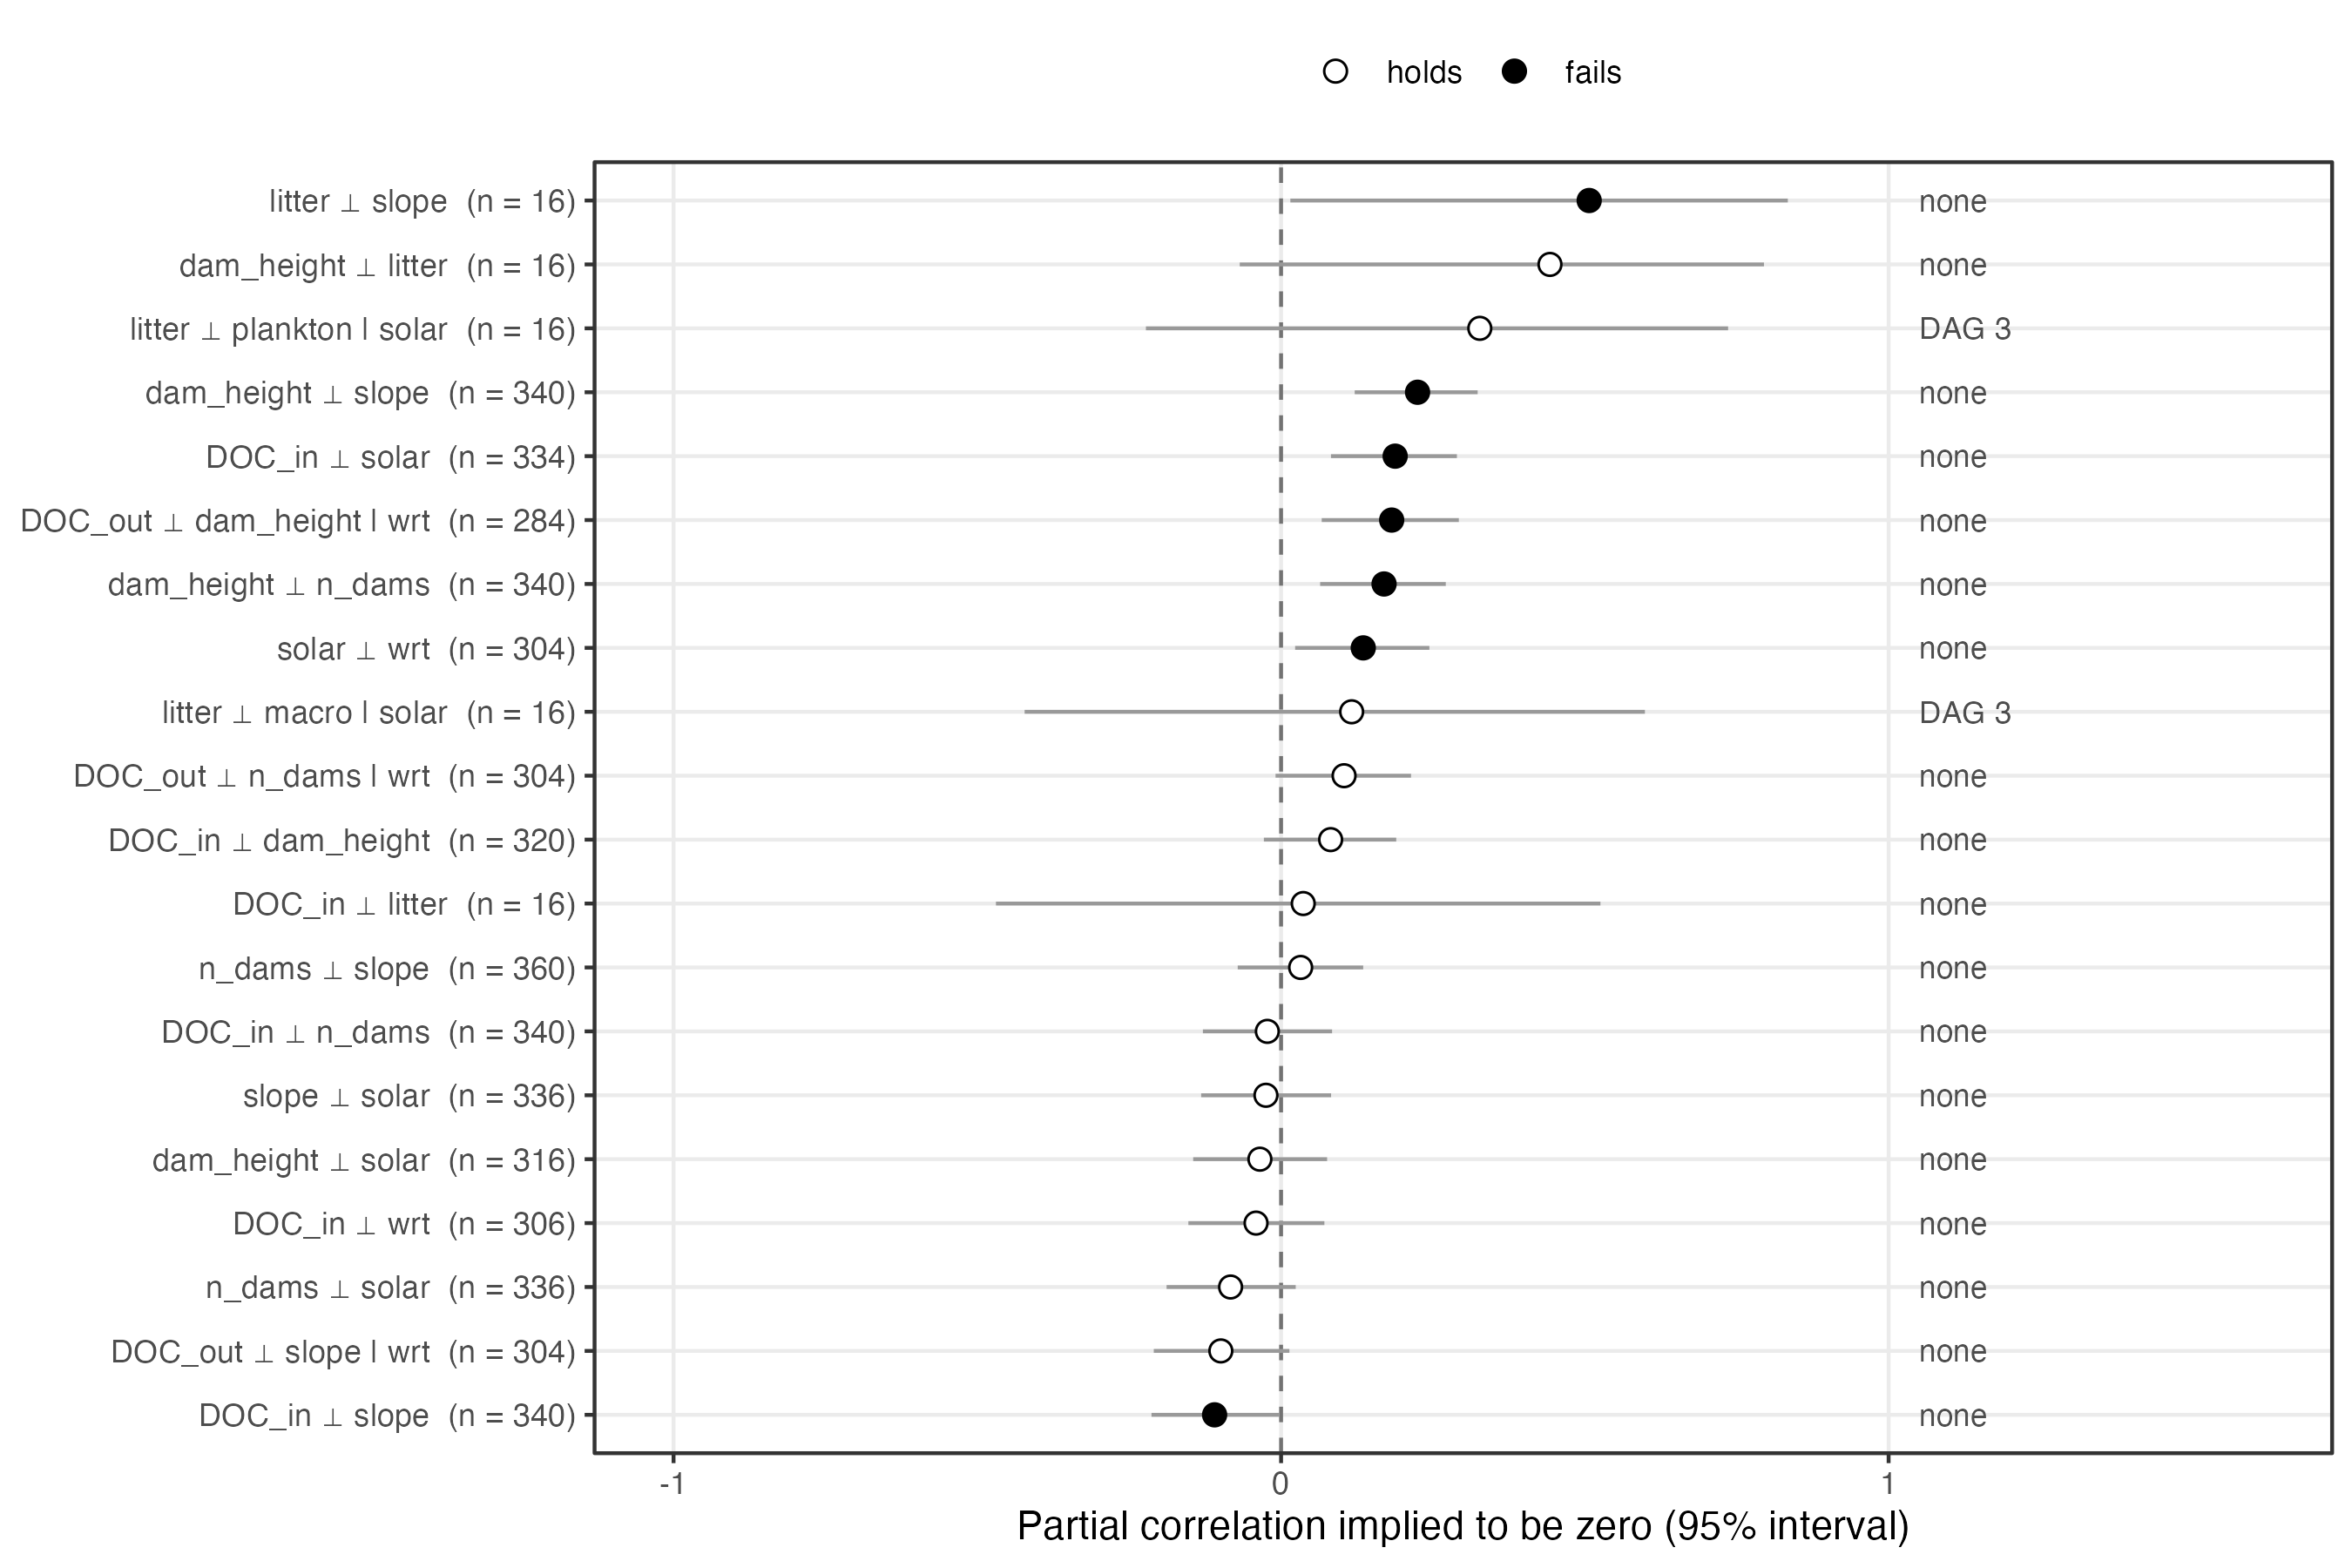
\includegraphics[width=\textwidth]{figures/media/figS10_dag_tests.png}
\caption{Conditional independencies implied by the reported structural causal model (DAG 0), tested on the data. Each row is one independence the model implies; the point is the partial correlation on the rows complete for the variables involved, with its 95\% interval and the number of samplings used. Filled points: the interval excludes zero (the independence fails). The right-hand label names the alternative structure(s) that would drop that independence, i.e.\ that a failure would support.}\label{fig:S10}
\end{figure}

\begin{figure}[!htb]
\centering
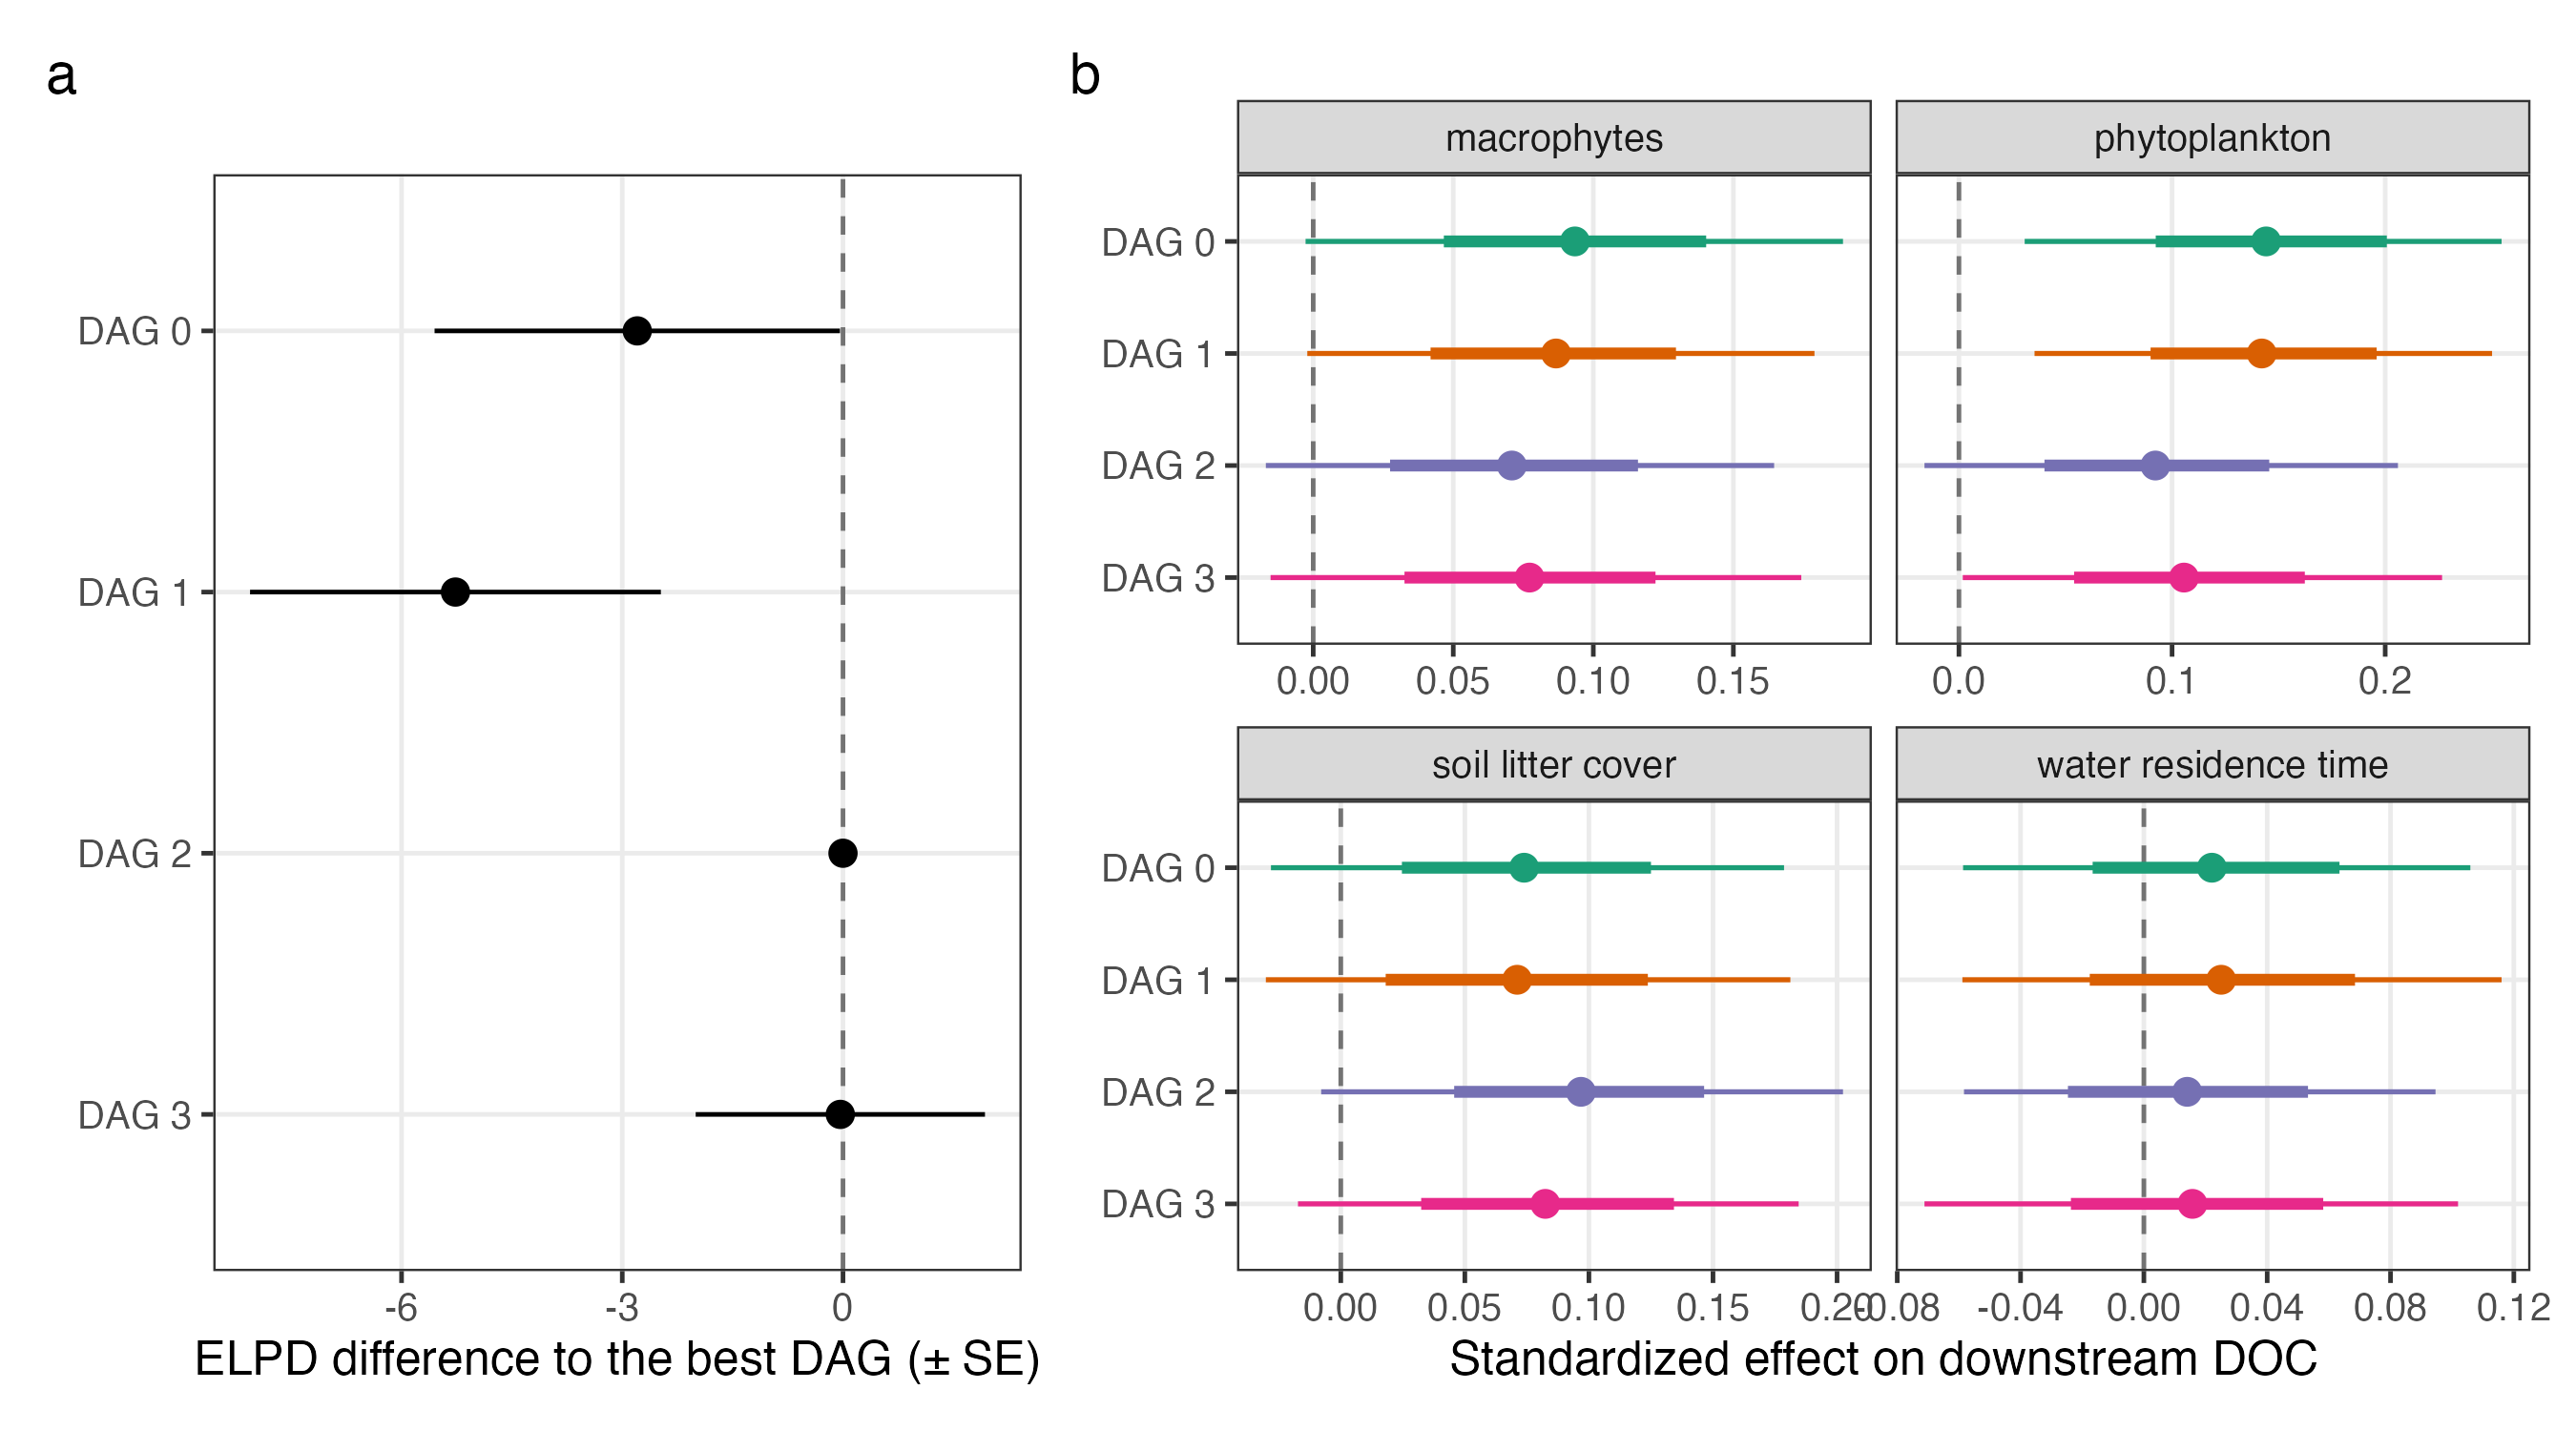
\includegraphics[width=\textwidth]{figures/media/figS11_dag_compare.png}
\caption{The four causal structures fitted as multivariate Bayesian models. a) Out-of-sample fit for downstream DOC by Pareto-smoothed importance-sampling leave-one-out cross-validation (PSIS-LOO): expected log predictive density relative to the best-fitting structure (0 = best), with standard error; a difference smaller than about 4 is not meaningful. b) The mediator effects on downstream DOC under each structure: posterior median with 66\% and 95\% credible intervals.}\label{fig:S11}
\end{figure}

\paragraph{Results.} Of the 20 conditional independencies the reported structure implies and that could be tested on the data, 7 fail; none of them is dropped by any of the three alternative DAGs, meaning none supports an alternative causal path over the reported one. The failures are confined to the exogenous drivers (e.g.\ upstream DOC, channel gradient and solar radiation), which share landscape causes that the SCM tolerates because none of them lies on a causal path to another (Figure~\ref{fig:S10}). No alternative DAG fits meaningfully better by PSIS-LOO: the nominally best structure is DAG 2 (direct solar~$\rightarrow$~downstream DOC path, estimate 0.11, 95\% BCI: 0.04; 0.18, $P(\beta>0) > 0.99$); the reported DAG 0 sits 2.8 ELPD below it (SE 2.8), DAG 3 (season) is statistically indistinguishable from the best ($-0.04$, SE 2.0), and DAG 1 (without the upstream-to-producer links) is 5.3 ELPD below the best (SE 2.8) -- in every case well below the usual threshold of 4 ELPD for a meaningful preference (max R-hat across the four fits: 1.02). Removing the two upstream-to-producer links (DAG 1) leaves the mediator effects on downstream DOC indistinguishable from the reported structure (Figure~\ref{fig:S11}b): the links matter for what predicts the producers, not for what the producers do to downstream DOC. These four DAGs do not exhaust the possible causal graphs, but the mediator effects reported in the main text are not an artefact of the particular arrows drawn among the tested alternatives.

\FloatBarrier
\section*{Robustness of the producer effects to unmeasured confounding}

The primary-producer effects on downstream DOC rest on the 16 streams where phytoplankton, macrophytes and litter cover were measured, all in summer. Following Cinelli and Hazlett (2020), we asked how strong an unobserved common cause of a producer and downstream DOC would have to be to erase the producer's effect, fitting the outcome as a linear model on these 16 streams (water residence time is absent there and could not be included), with solar radiation as a benchmark covariate of known strength.

\begin{figure}[!htb]
\centering
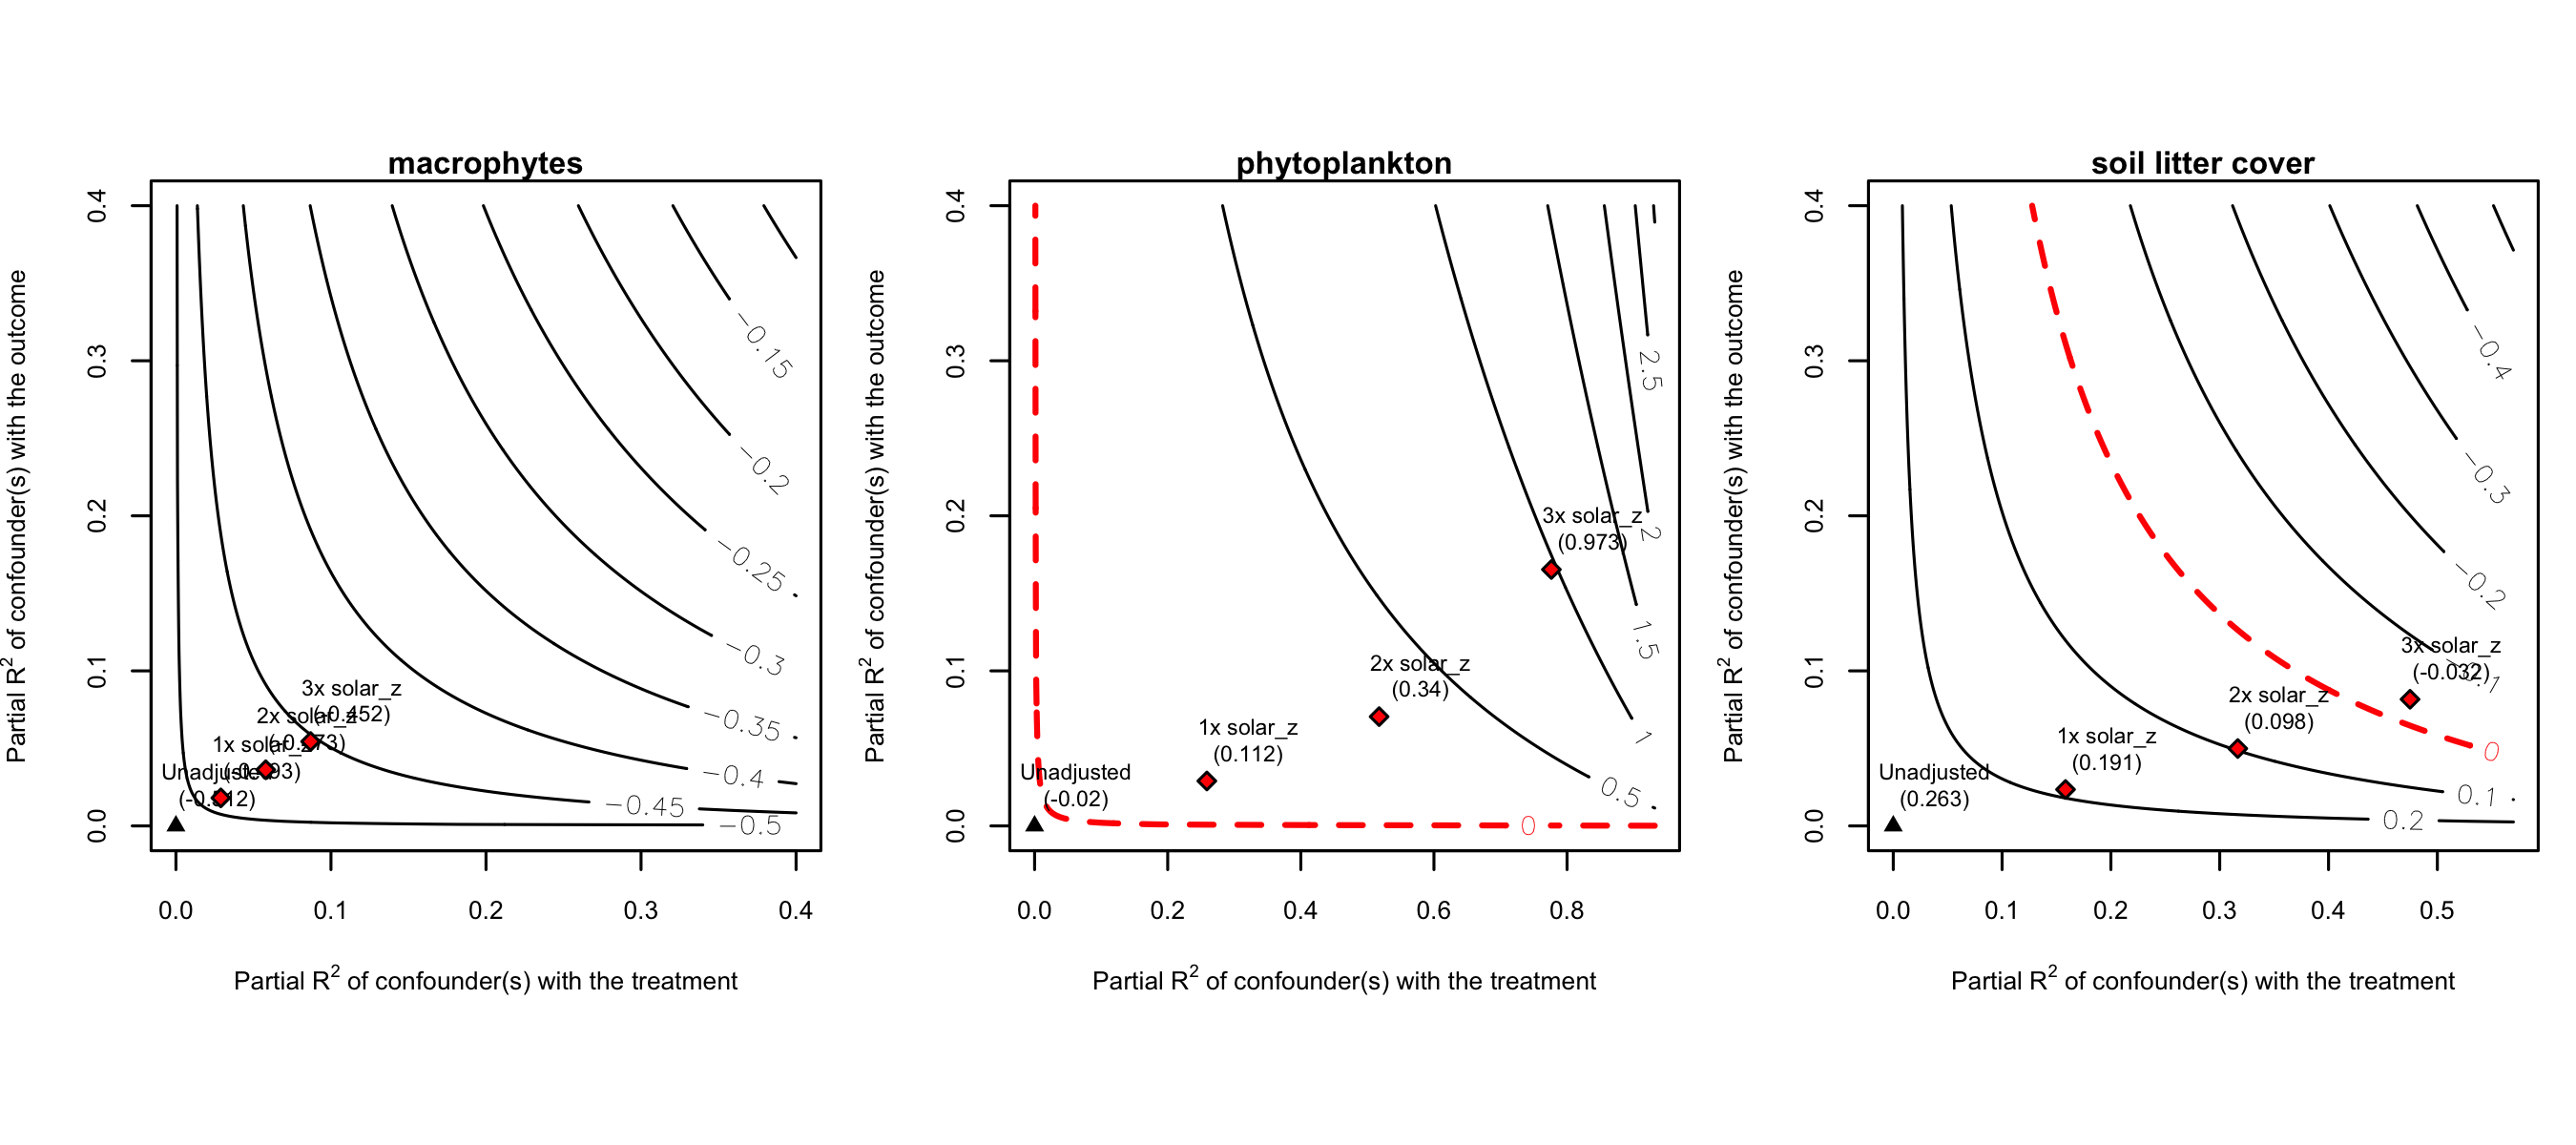
\includegraphics[width=\textwidth]{figures/media/figS12_sensemakr.png}
\caption{Robustness of each producer $\rightarrow$ downstream DOC path to an unmeasured confounder. Contours: the adjusted effect of the producer on downstream DOC for a confounder with the given partial $R^2$ with the producer (x-axis) and with downstream DOC (y-axis); the triangle is the unadjusted estimate; the red marks are confounders 1$\times$, 2$\times$ and 3$\times$ as strong as solar radiation. Linear outcome equation on the 16 producer streams (summer). This linear fit does not carry the priors, the measurement error or the water-residence-time path of the SCM; it is the sensitivity of the raw 16-stream relationship.}\label{fig:S12}
\end{figure}

\paragraph{Results.} The raw 16-stream relationship is not the SCM's: the linear-model estimates are $-0.51$ (macrophytes), $-0.02$ (phytoplankton) and 0.26 (litter), against $+0.09$, $+0.14$ and $+0.07$ in the SCM. The SCM's positive producer effects are therefore carried substantially by the informative priors (Normal(0.2, 0.075) on each producer path) and by the hierarchical structure, not by these 16 samplings alone -- the single most important sensitivity result of this appendix section, confirmed independently by the prior-sensitivity check below. The robustness values (the confounder strength needed to erase the raw effect) are 0.45 for macrophytes, 0.21 for litter and 0.01 for phytoplankton; solar radiation, the strongest measured covariate, explains only 3--26\% of the residual variance of any producer, so a confounder several times stronger than solar would be needed to remove the macrophyte or litter relationship, and almost none to remove the phytoplankton one. Water residence time could not be assessed this way, as it was never measured at a producer stream. The producer~$\rightarrow$~DOC paths are therefore consistent with the literature-based priors and not overturned by plausible confounding, but with 16 summer samplings they remain prior-informed estimates rather than data-driven ones.

\FloatBarrier
\section*{Falsification tests and a placebo outcome}

The SCM implies that some relationships must be absent: if they were present, either the model or the data would be wrong somewhere. We tested three such implied nulls among the exogenous drivers, and one placebo outcome, upstream DOC, which lies above the dams and cannot be causally affected by beaver-engineering; if the number of dams, the dam height or the water residence time ``predicted'' upstream DOC, it would reveal a confounder (a landscape gradient setting both the dams and the DOC).

\begin{figure}[!htb]
\centering
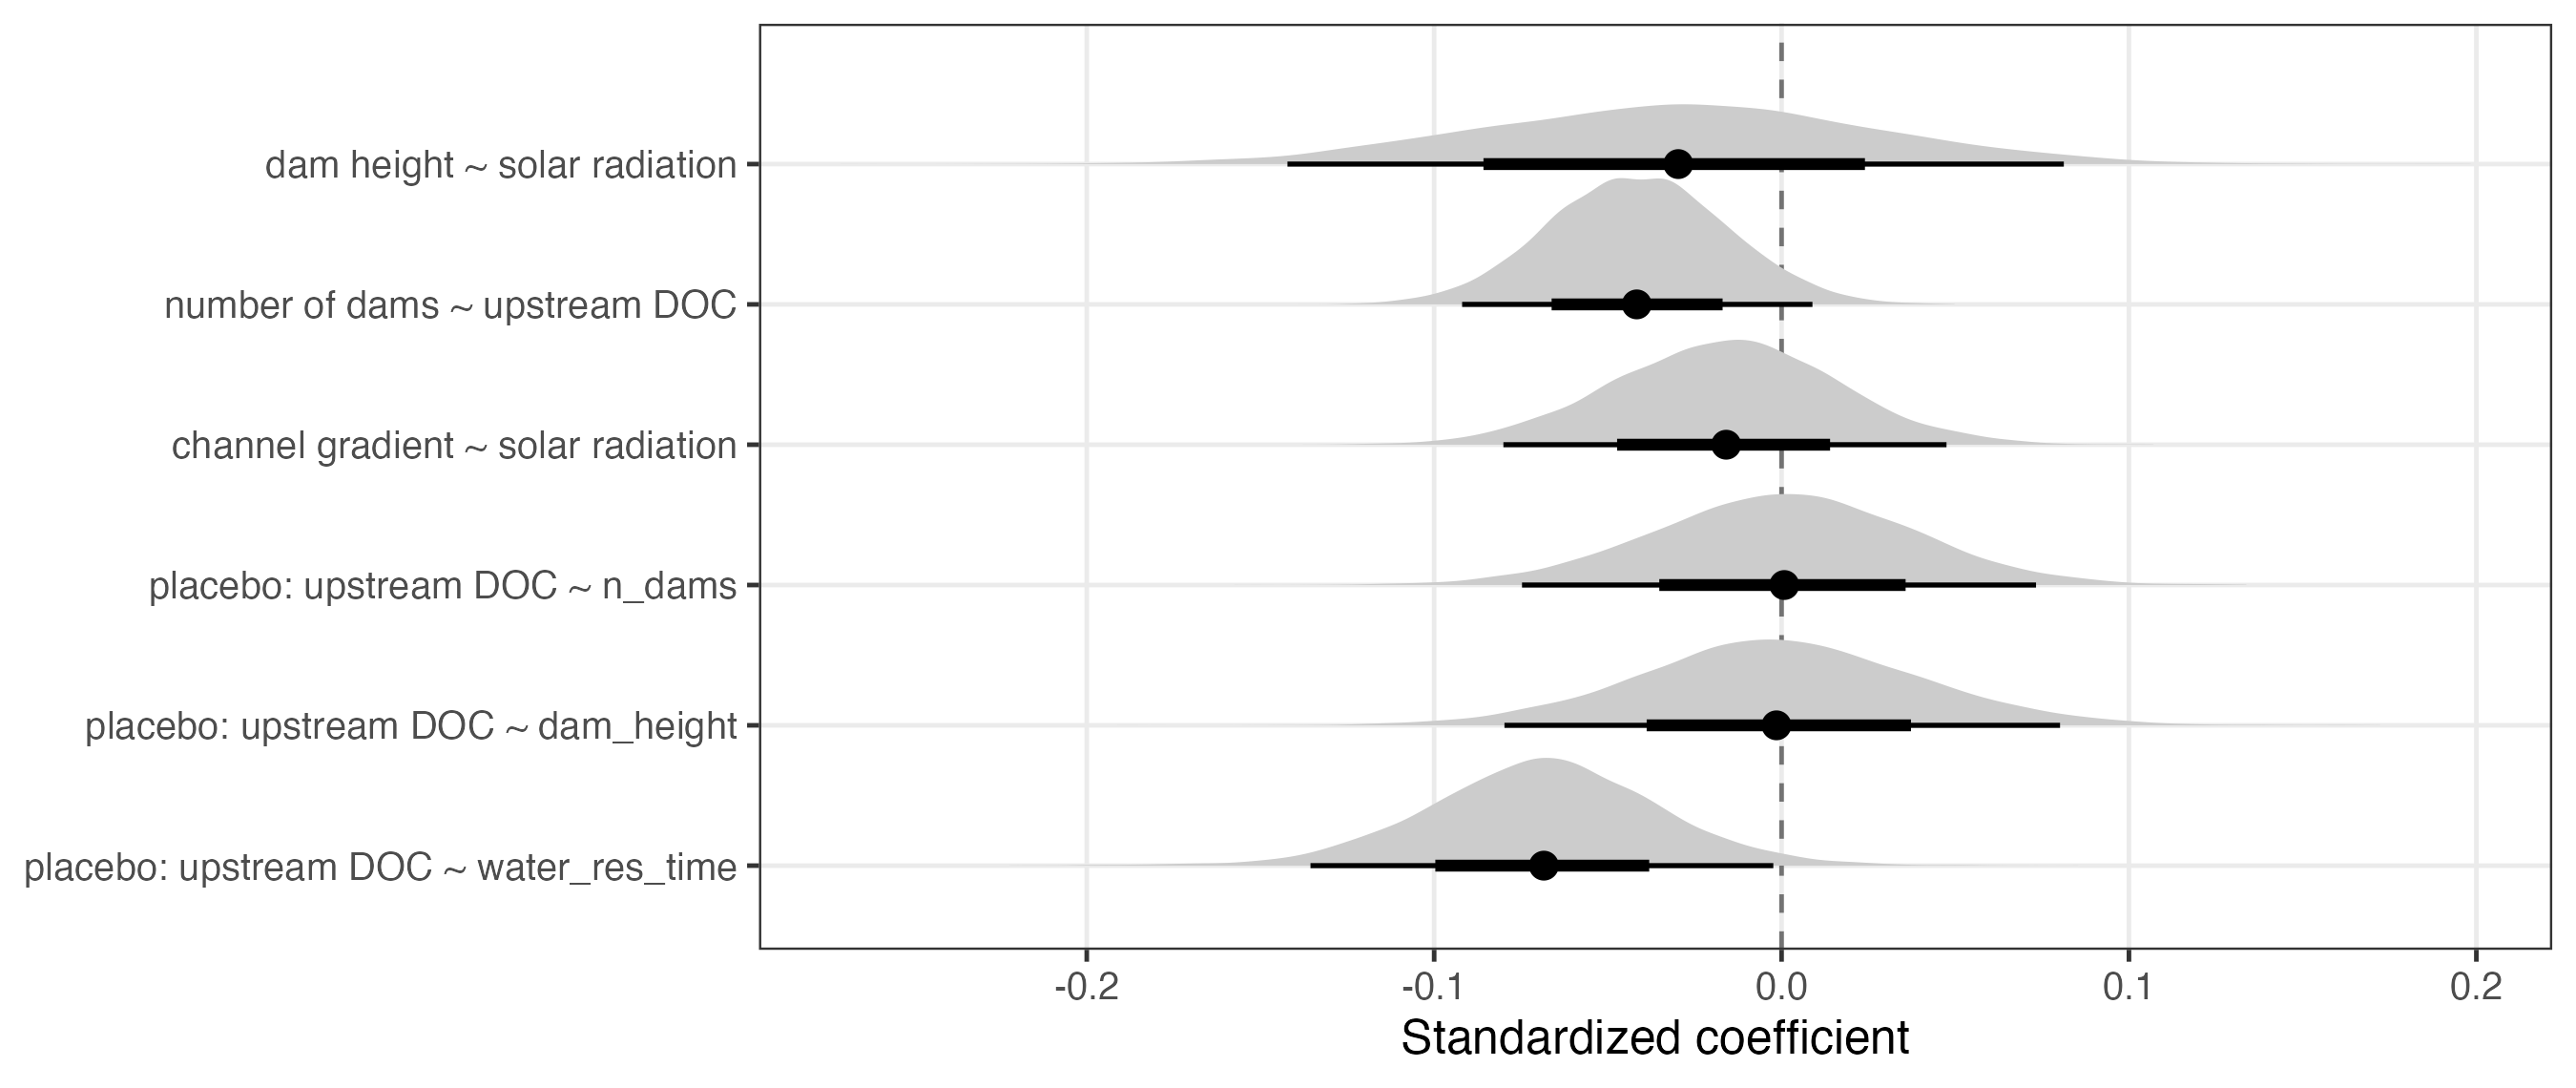
\includegraphics[width=\textwidth]{figures/media/figS13_negative_controls.png}
\caption{Relationships the structural causal model says must be null. Posterior distributions of the standardized coefficients of four Bayesian Student-$t$ regressions on all samplings (Normal(0,1) priors on the slopes); point: median, bars: 66\% and 95\% credible intervals; dashed line: zero. The last three rows are the placebo outcome, upstream DOC regressed on the beaver-engineering variables, which cannot causally affect it.}\label{fig:S13}
\end{figure}

\paragraph{Results.} All three implied nulls among the exogenous drivers were consistent with zero: channel gradient $\sim$ solar radiation $-0.02$ (95\% BCI: $-0.08$; 0.05, $P(\beta>0)=0.30$); dam height $\sim$ solar radiation $-0.03$ ($-0.14$; 0.08, $P(\beta>0)=0.29$); number of dams $\sim$ upstream DOC $-0.04$ ($-0.09$; 0.01, $P(\beta>0)=0.05$). Of the placebo regressions of upstream DOC on the beaver-engineering variables, dam height and number of dams were indistinguishable from zero, but water residence time showed a small, credibly non-zero association ($-0.07$, 95\% BCI: $-0.14$; $-0.00$): any confounding of the dams~$\rightarrow$~residence-time~$\rightarrow$~DOC chain by the catchment's DOC regime is therefore at most of that size, an order of magnitude below the inheritance slope. A failed null among the exogenous drivers would mean those drivers share a landscape cause -- which the SCM tolerates, because they are not on a causal path to one another -- but a reader should know it; a failed placebo would mean the beaver-engineering variables are confounded with the catchment's DOC regime, which the result above rules out beyond a small margin.

\FloatBarrier
\section*{Prior sensitivity and spatial autocorrelation of the residuals}

\begin{figure}[!htb]
\centering
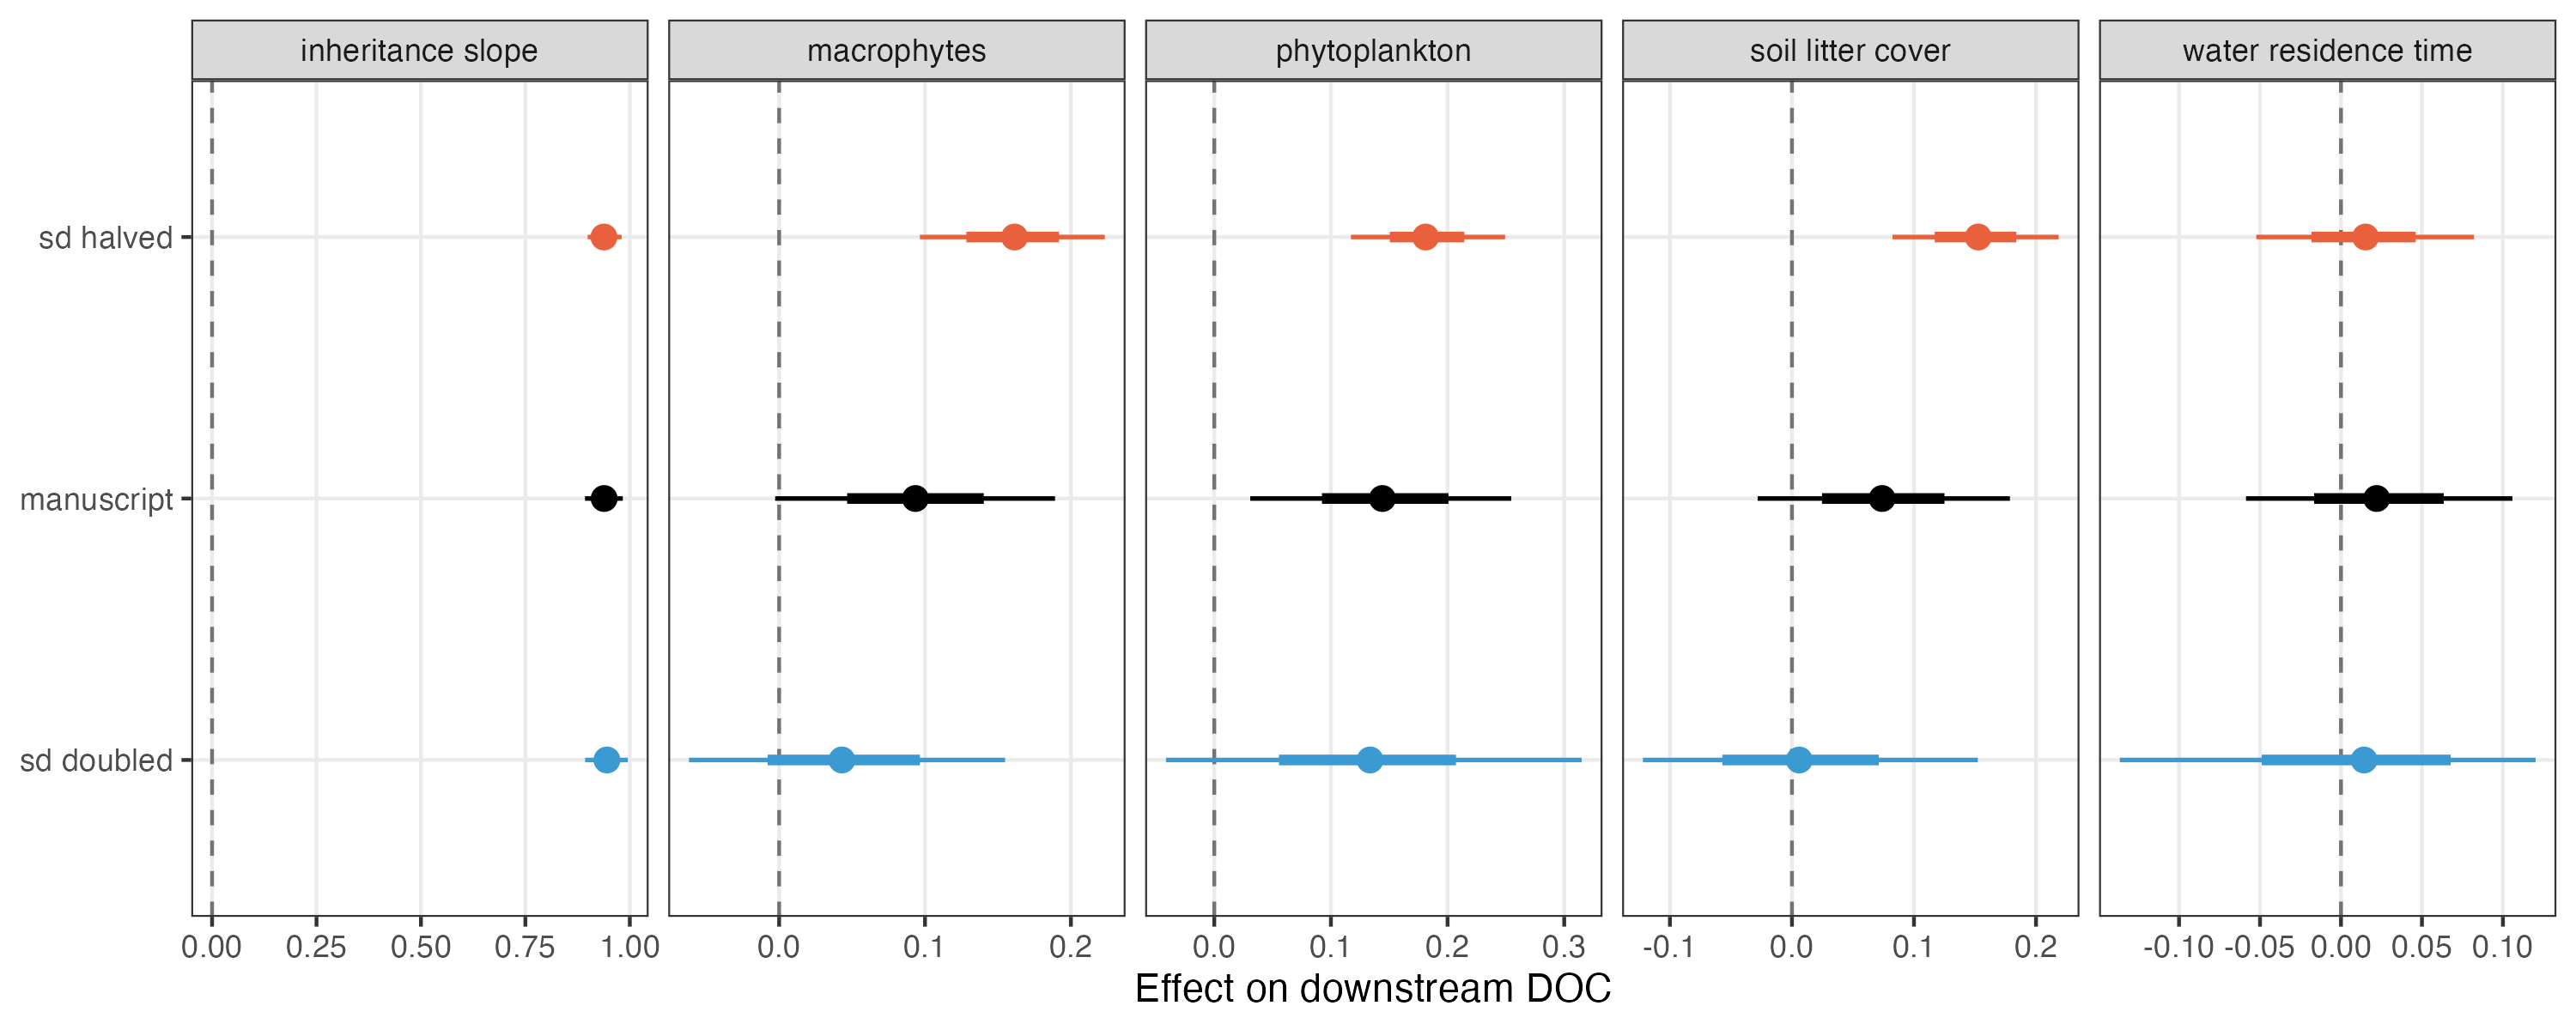
\includegraphics[width=\textwidth]{figures/media/figS14_prior_sens.png}
\caption{Prior sensitivity. Mediator effects on downstream DOC when the standard deviation of every informative prior is halved, kept as in the manuscript, or doubled; posterior median with 66\% and 95\% credible intervals. A path whose estimate follows the prior scale is prior-driven; a path that stays put is data-driven.}\label{fig:S14}
\end{figure}

\begin{figure}[!htb]
\centering
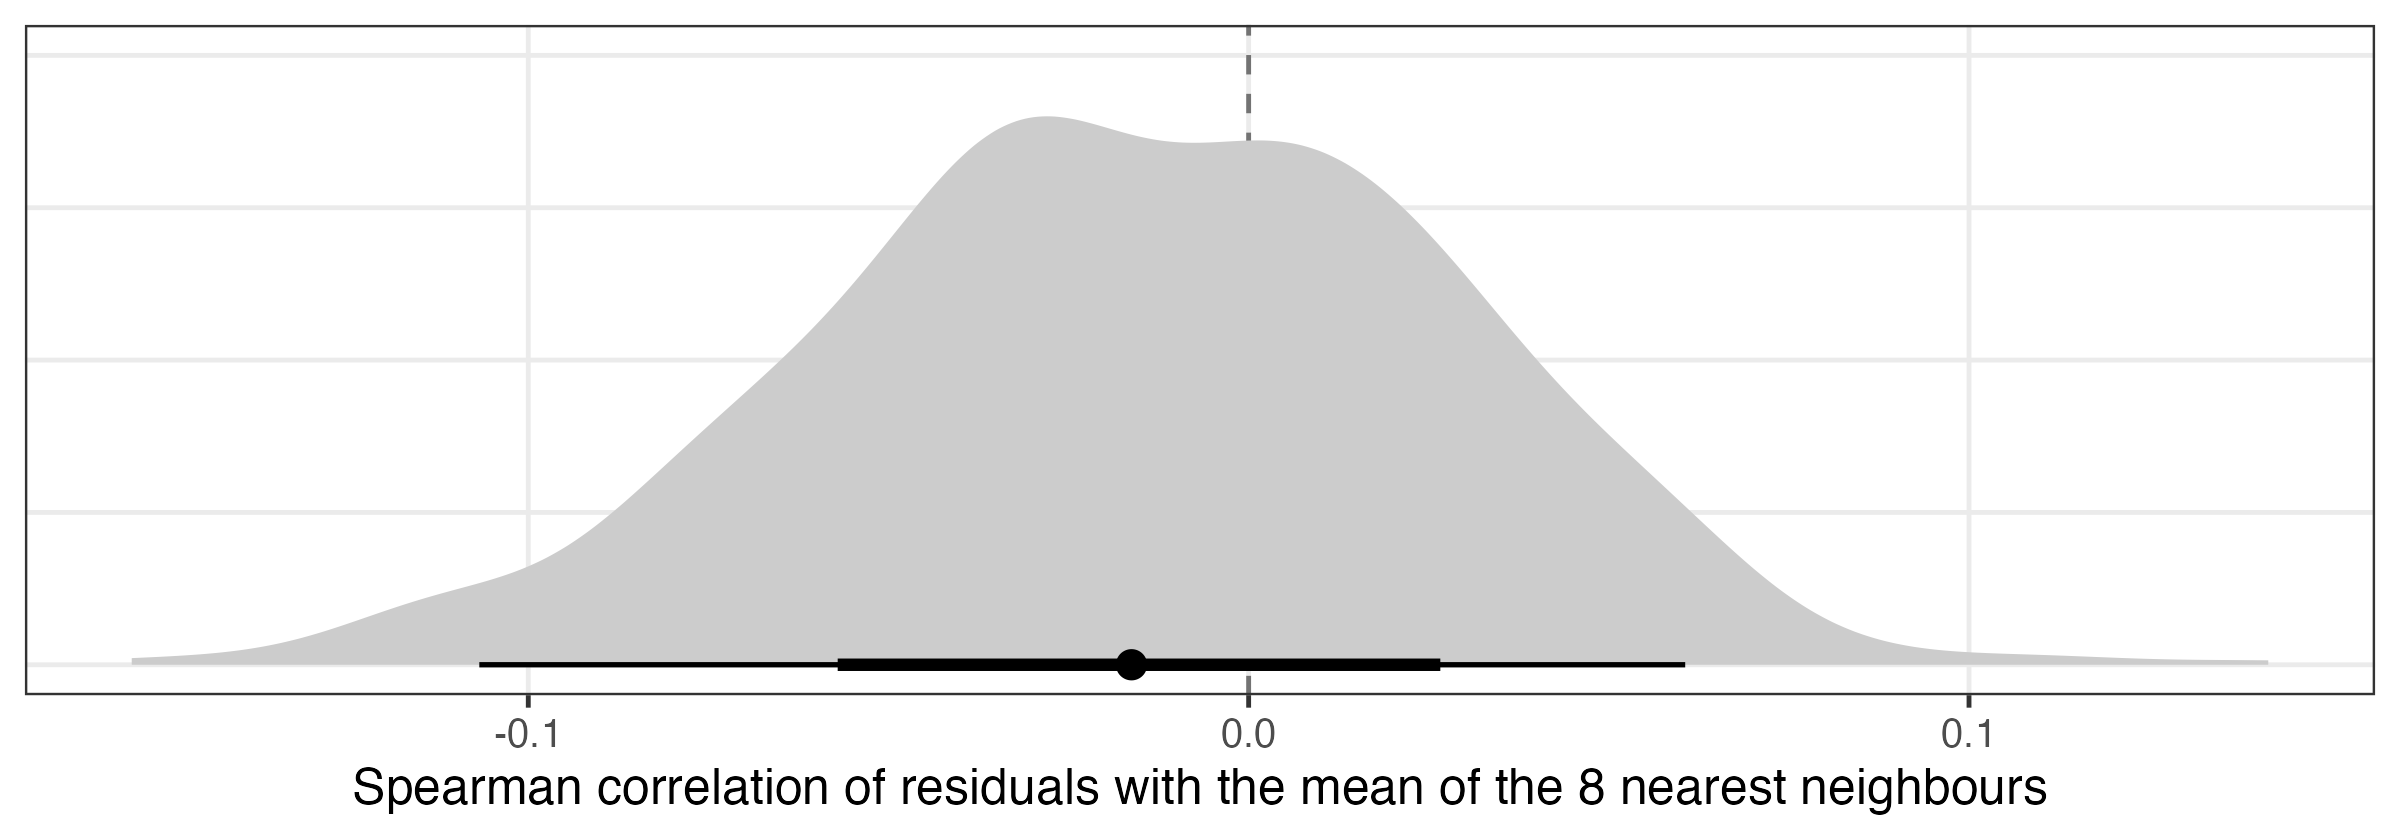
\includegraphics[width=0.75\textwidth]{figures/media/figS15_spatial_resid.png}
\caption{Spatial autocorrelation of the residuals of downstream DOC. For each posterior draw, the Spearman correlation between each sampling's residual (observed minus expected downstream DOC) and the mean residual of its 8 nearest neighbouring samplings, using the stream coordinates; point: median, bars: 66\% and 95\% credible intervals; dashed line: no spatial autocorrelation.}\label{fig:S15}
\end{figure}

\paragraph{Results.} The inheritance slope did not move when every informative prior's standard deviation was halved or doubled (0.94, 0.94 and 0.95 respectively). The producer paths moved with the prior: the largest shift was soil litter cover, from 0.15 (sd halved) to 0.01 (sd doubled); phytoplankton kept its sign throughout (0.13 with sd doubled), while macrophytes and litter followed the prior more closely -- the same conclusion as the unmeasured-confounding check above, reached from the other side. No spatial autocorrelation remained in the residuals of downstream DOC once upstream DOC and the drivers were in the model: the neighbour correlation was $-0.02$ (95\% BCI: $-0.11$; 0.06), indicating that the stream random effect accounts for spatial structure and that no explicit spatial term is needed.

\FloatBarrier
\section*{Causal knowledge analysis}

Table~\ref{tab:S2} summarizes the qualitative frame the quantitative checks above sit in, following Grace's causal-knowledge analysis.

\begin{center}
\begin{small}
\begin{longtable}{|>{\raggedright\arraybackslash}p{0.24\textwidth}|>{\raggedright\arraybackslash}p{0.5\textwidth}|>{\raggedright\arraybackslash}p{0.16\textwidth}|}
\caption{Causal knowledge analysis of the beaver--DOC system.}\label{tab:S2}\\
\hline
\textbf{Question} & \textbf{Answer for the beaver--DOC system} & \textbf{Where addressed} \\ \hline
\endfirsthead
\multicolumn{3}{l}{\small\textit{Table S2 (continued)}}\\
\hline
\textbf{Question} & \textbf{Answer for the beaver--DOC system} & \textbf{Where addressed} \\ \hline
\endhead
\multicolumn{3}{r}{\small\textit{continued on next page}}\\
\endfoot
\endlastfoot
1. What causal quantity is sought? & The local modification that beaver-engineering adds to downstream DOC, decomposed into its hydrological and biological pathways; and its size relative to the inherited seasonal contrast. & Drivers (SCM), magnitude ($R_s$, $G$) \\ \hline
2. What is the causal system and its boundary? & The beaver-engineered stream from the first to the last dam; inputs are upstream DOC, solar radiation, channel gradient, dams; the floodplain and the catchment are outside, represented by upstream DOC and $S$. & Figure 1b, DAG (Figure 4), main document \\ \hline
3. What is assumed about the structure (arrows present)? & Dams $\rightarrow$ residence time $\rightarrow$ producers $\rightarrow$ DOC; solar $\rightarrow$ producers $\rightarrow$ DOC; litter $\rightarrow$ DOC; upstream DOC inherited with slope near 1; upstream DOC $\rightarrow$ macrophytes (and, more weakly, $\rightarrow$ phytoplankton). & Table~S1 (13 hypotheses); this appendix \\ \hline
4. What is assumed absent (arrows omitted, no confounding)? & No direct solar $\rightarrow$ DOC, no season confounding, no unmeasured common cause of producers and DOC. & None of the omitted arrows is supported (above); placebo and implied nulls above \\ \hline
5. How are the effects identified? & By the SCM's adjustment sets, with measurement error on every concentration and imputation of missing predictors; the inheritance slope is estimated, not assumed. & Methods; robustness to slope = 1 (Methods) \\ \hline
6. Is the data adequate for the structure? & 158 streams for the inheritance and the direction; 16 summer streams for the producers, with no water residence time at those streams. The producer paths are the weak point. & Unmeasured-confounding and prior-sensitivity checks above \\ \hline
7. How sensitive are the conclusions? & Inheritance, the null average and the heterogeneity are robust to structure, priors, outcome parameterization and space; the sign of each producer path follows the prior scale. & This appendix, in full \\ \hline
8. To what does the result transport? & To Swiss low-order single-thread streams with 1--19 dams; downstream DOC at an unseen stream is predictable, the sign of the local change is not. & Model validation (Methods) \\ \hline
\end{longtable}
\end{small}
\end{center}

\FloatBarrier
\section*{References}
\begin{itemize}\setlength\itemsep{2pt}
\item[] Wegener P, Covino T, and Wohl E. 2017. Beaver-mediated lateral hydrologic connectivity, fluvial carbon and nutrient flux, and aquatic ecosystem metabolism. Water Resources Research \textbf{53}: 4606--23.
\item[] Wohl E. 2021. An integrative conceptualization of floodplain storage. Reviews of Geophysics \textbf{59}: e2020RG000724.
\item[] Bencala KE and Walters RA. 1983. Simulation of solute transport in a mountain pool-and-riffle stream: A transient storage model. Water Resources Research \textbf{19}: 718--24.
\item[] Abbasi M, Peacock M, Drakare S, et al. 2024. \href{https://doi.org/10.1016/j.watres.2024.121910}{Water residence time is an important predictor of dissolved organic matter composition and drinking water treatability}. Water Research \textbf{260}: 121910.
\item[] Aitkenhead JA, Hope D, and Billett MF. 1999. \href{https://doi.org/10.1002/(SICI)1099-1085(19990615)13:8\%3C1289::AID-HYP766\%3E3.0.CO;2-M}{The relationship between dissolved organic carbon in stream water and soil organic carbon pools at different spatial scales}. Hydrological Processes \textbf{13}: 1289--302.
\item[] Cincotta MM, Perdrial JN, Shavitz A, et al. 2019. \href{https://doi.org/10.3389/fenvs.2019.00172}{Soil aggregates as a source of dissolved organic carbon to streams: An experimental study on the effect of solution chemistry on water extractable carbon}. Frontiers in Environmental Science \textbf{7}.
\item[] Cinelli C and Hazlett C. 2020. \href{https://doi.org/10.1111/rssb.12348}{Making sense of sensitivity: Extending omitted variable bias}. Journal of the Royal Statistical Society Series B: Statistical Methodology \textbf{82}: 39--67.
\item[] Dittbrenner BJ, Schilling JW, Torgersen CE, and Lawler JJ. 2022. \href{https://doi.org/10.1002/ecs2.4168}{Relocated beaver can increase water storage and decrease stream temperature in headwater streams}. Ecosphere \textbf{13}: e4168.
\item[] Feuchtmayr H, Moran R, Hatton K, et al. 2009. \href{https://doi.org/10.1111/j.1365-2664.2009.01644.x}{Global warming and eutrophication: effects on water chemistry and autotrophic communities in experimental hypertrophic shallow lake mesocosms}. Journal of Applied Ecology \textbf{46}: 713--23.
\item[] Finger D, Schmid M, and Wüest A. 2007. \href{https://doi.org/10.1029/2007WR005868}{Comparing effects of oligotrophication and upstream hydropower dams on plankton and productivity in perialpine lakes}. Water Resources Research \textbf{43}.
\item[] Hayes AF. 2018. Introduction to Mediation, Moderation, and Conditional Process Analysis: A Regression-Based Approach, 2nd edn. New York: Guilford Press.
\item[] Gessner MO, Chauvet E, and Dobson M. 1999. \href{https://doi.org/10.2307/3546505}{A perspective on leaf litter breakdown in streams}. Oikos \textbf{85}: 377--84.
\item[] Jepsen SM, Harmon TC, Sadro S, et al. 2019. \href{https://doi.org/10.1016/j.scitotenv.2018.11.392}{Water residence time (age) and flow path exert synchronous effects on annual characteristics of dissolved organic carbon in terrestrial runoff}. Science of The Total Environment \textbf{656}: 1223--37.
\item[] Johnston CA. 2014. \href{https://doi.org/10.1016/j.geoderma.2013.08.025}{Beaver pond effects on carbon storage in soils}. Geoderma \textbf{213}: 371--8.
\item[] Larson JH, Frost PC, Zheng Z, et al. 2007. \href{https://doi.org/10.4319/lo.2007.52.1.0060}{Effects of upstream lakes on dissolved organic matter in streams}. Limnology and Oceanography \textbf{52}: 60--9.
\item[] Majerova M, Neilson BT, Schmadel NM, et al. 2015. \href{https://doi.org/10.5194/hess-19-3541-2015}{Impacts of beaver dams on hydrologic and temperature regimes in a mountain stream}. Hydrology and Earth System Sciences \textbf{19}: 3541--56.
\item[] Manolaki P, Olesen A, Hvidt BG, et al. 2021. \href{https://doi.org/10.1051/kmae/2021020}{Investigating emergent macrophytes establishment rate and propagation towards constructed wetlands efficacy optimization}. Knowledge \& Management of Aquatic Ecosystems 23.
\item[] McGuire KJ, McDonnell JJ, Weiler M, et al. 2005. \href{https://doi.org/10.1029/2004WR003657}{The role of topography on catchment-scale water residence time}. Water Resources Research \textbf{41}.
\item[] Nyssen J, Pontzeele J, and Billi P. 2011. \href{https://doi.org/10.1016/j.jhydrol.2011.03.008}{Effect of beaver dams on the hydrology of small mountain streams: Example from the chevral in the ourthe orientale basin, ardennes, belgium}. Journal of Hydrology \textbf{402}: 92--102.
\item[] Reitsema RE, Meire P, and Schoelynck J. 2018. \href{https://doi.org/10.3389/fpls.2018.00629}{The future of freshwater macrophytes in a changing world: Dissolved organic carbon quantity and quality and its interactions with macrophytes}. Frontiers in Plant Science \textbf{9}.
\item[] Reynolds CS. 2006. \href{https://doi.org/10.1017/CBO9780511542145}{The ecology of phytoplankton}. Cambridge: Cambridge University Press.
\item[] Sell AF and Overbeck J. 1992. \href{https://doi.org/10.1093/plankt/14.9.1199}{Exudates: Phytoplankton-bacterioplankton interactions in pluβsee}. Journal of Plankton Research \textbf{14}: 1199--215.
\item[] Søndergaard M, Riemann B, and Jørgensen NOG. 1985. \href{https://doi.org/10.2307/3565567}{Extracellular organic carbon (EOC) released by phytoplankton and bacterial production}. Oikos \textbf{45}: 323--32.
\item[] SwissTopo. 2024. \href{https://www.swisstopo.admin.ch/en/landscape-model-swisstlm3d}{swissTLM3D -- topographic landscape model}.
\item[] Westbrook CJ, Cooper DJ, and Baker BW. 2006. \href{https://doi.org/10.1029/2005WR004560}{Beaver dams and overbank floods influence groundwatersurface water interactions of a Rocky Mountain riparian area}. Water Resources Research \textbf{42}.
\item[] Wohl E. 2013. \href{https://doi.org/10.1002/grl.50710}{Landscape-scale carbon storage associated with beaver dams}. Geophysical Research Letters \textbf{40}: 3631--6.
\end{itemize}
\end{document}
